\documentclass[11pt,a4paper]{article}
% allow both latex and PDFlatex compatibility  (from pdfTeX FAQ)
\usepackage{hyperlatex}

\usepackage{pifont}
\usepackage{amsmath}
\usepackage{amssymb}
%\usepackage{psfig}
\usepackage{array}
\usepackage{supertabular}
%\usepackage{fancyheadings}
\usepackage{here}
\usepackage{eepic,epic}
%\usepackage{pslatex} % devrait corriger le pb de fontes dans les pdfs mais le fichier produit n'est pas beau
\usepackage[english]{babel}
\usepackage{alltt}
% \usepackage{textcomp]


\texonly{\newcommand{\tilda}{{$_{\widetilde{\ }}$}}}
%\texonly{\newcommand{\tilda}{{\~{}}}}
\htmlonly{\newcommand{\tilda}{\verb+~+}}

\texonly{\usepackage{graphicx}
\usepackage{makeidx}
\usepackage[pdftex,pageanchor=true,hyperindex=true,pagebackref=true,pdfhighlight=/O,pdfauthor={Yves Renard}]{hyperref}%pour le pdf
\usepackage{xspace} % insere un espace si necessaire 
\usepackage{underscore}

\newcommand{\ds}{\displaystyle}
\oddsidemargin -0.9cm
\evensidemargin -0.9cm
\topmargin -1cm
\textheight 22.5cm
\textwidth 17.6cm
\headheight 1.0cm
}
\makeindex


\T \newcommand{\Reel}{{\rm I\hspace{-0.15em}R}}
\W \newcommand{\Reel}{\htmlsym{real}}
\T \newcommand{\ds}{\displaystyle}
\W \newcommand{\ds}{}
\newcommand{\Frac}[2]{{\ds \frac{\ds #1}{\ds #2}}}

\T \newcommand{\icgraphic}[3] { \includegraphics[width=#1]{#2.pdf} }
\W \newcommand{\icgraphic}[3] { \htmlimg{#2.png}{#3} }

\T \newcommand{\equat}[1] { \begin{equation*} #1 \end{equation*} }
\W \newcommand{\equat}[1] { \begin{center} $ #1 $ \end{center} }


% \W .. is equivalent to \htmlonly{..}
\W \newcommand{\HlxIcons}{./}
%\W \usepackage{frames} % navigation panel
\W \htmldirectory{getfem_project}
\W \htmlname{getfem_project}
\W \setcounter{htmldepth}{2}
\W \setcounter{htmlautomenu}{2}
\W \renewcommand{\HlxMeta}{\xml{META description="getfem++ user manual"}}
\htmlonly{%
  \htmlpanelfield{Index}{getfem_project}
  \htmlcss{docstyle.css}
  \newcommand{\text}[1]{\mathrm{#1}}
  \newcommand{\WEB}[2]{\xlink{#2}{#1}}
  \newcommand{\nabla}{\htmlsym{nabla}} % renamed \xmlent by lastest version of hyperlatex
  \newcommand{\ell}{\htmlsym{tau}}
  \newcommand{\lambda}{\htmlsym{lambda}}
  \newcommand{\varepsilon}{\htmlsym{epsilon}}
  \newcommand{\phi}{\htmlsym{phi}}
  \newcommand{\varphi}{\htmlsym{phi}}
  \newcommand{\psi}{\htmlsym{psi}}
  \newcommand{\sigma}{\htmlsym{sigma}}
  \newcommand{\nu}{\htmlsym{nu}}
  \newcommand{\beta}{\htmlsym{beta}}
  \newcommand{\gamma}{\htmlsym{gamma}}
  \newcommand{\alpha}{\htmlsym{alpha}}
  \newcommand{\Gamma}{\htmlsym{Gamma}}
  \newcommand{\Delta}{\htmlsym{Delta}}
  \newcommand{\delta}{\htmlsym{delta}}
  \newcommand{\Omega}{\htmlsym{Omega}}
  \newcommand{\omega}{\htmlsym{omega}}
  \newcommand{\otimes}{\htmlsym{otimes}}
  \newcommand{\prod}{\htmlsym{Pi}}
  \newcommand{\tau}{\htmlsym{tau}}
  \newcommand{\partial}{\htmlsym{part}}
  \newcommand{\sum}{\htmlsym{sum}}
  \newcommand{\subset}{\htmlsym{sub}}
  \newcommand{\int}{{\Large\htmlsym{int}}}
}
\texonly{
  \newcommand{\WEB}[2]{\href{#1}{#2}}
}
\T \newcommand{\Div}{\textrm{div}}
\W \newcommand{\Div}{div}
\T \newcommand{\Grad}{\textrm{grad}}
\W \newcommand{\Grad}{grad}
\T \newcommand{\Rot}{\textrm{curl}}
\W \newcommand{\Rot}{curl}

\W \newcommand{\gf}{Getfem\mbox{++}\hspace{0.01em}}
\T \newcommand{\gf}{{\sc Getfem++}\xspace}
\W \newcommand{\gmm}{Gmm\mbox{++}\hspace{0.01em}}
\T \newcommand{\gmm}{{\sc Gmm++}\xspace}

\W \newcommand{\newpage}{}
\W \newcommand{\hspace}[1]{ }
\W \newcommand{\left}{} % pour les left\(i\right) 
\W \newcommand{\right}{}
\W \newenvironment{alltt}{\begin{example}}{\end{example}}
\T \newenvironment{cppcode}{\begin{alltt}}{\end{alltt}}
\W \newenvironment{cppcode}{\begin{rawxml}<div class="cppcode">\end{rawxml}\begin{example}}{\end{example}\begin{rawxml}</div>\end{rawxml}}

\T \newcommand{\cpp}[1]{\texttt{#1}}
\T \newcommand{\filename}[1]{\texttt{#1}}

%doxfilename and doxref : used by doxygenlinks.tex
\T \newcommand{\doxfilename}[2]{\texttt{#1}}
\T \newcommand{\doxref}[2]{\cpp{#1}}

\W \newcommand{\cpp}[1]{\xmlattributes*{tt}{class="inlinecppcode"}\texttt{#1}}
\W \newcommand{\filename}[1]{\xmlattributes*{tt}{style="color:red"}\texttt{#1}}
\W \newcommand{\doxfilename}[2]{\xmlattributes*{tt}{class="inlinecppcode"}\texttt{\WEB{../getfem_reference/#2.html}{#1}}\xspace}
\W \newcommand{\doxref}[2]{\xmlattributes*{tt}{class="inlinecppcode"}\texttt{\WEB{../getfem_reference/#2.html}{#1}}\xspace}

\T \newenvironment{ctableau}[2]{\begin{center}\begin{supertabular}{#1}}{\end{supertabular}\end{center}}
\W \newenvironment{ctableau}[2]{\xmlattributes*{table}{border=1 align="center"}\begin{tabular}{#2}}{\end{tabular}}

\newcommand{\WEBB}[1]{\WEB{#1}{#1}}

\texonly{
  \newcommand{\femtab}[9]{
    \begin{center}
      \begin{tabular}{|m{16.109cm}|} \hline
        {\bf #1}\\
        {\tt #2} 
      \end{tabular} \\ \vspace{-0.12em} 
      \begin{tabular}{|m{2cm}|m{2cm}|m{2.5cm}|m{1.5cm}|m{1.5cm}|m{2cm}|m{2cm}|} \hline 
        Degree & dimension & d.o.f. number & class & vectorial & \mbox{$\tau$-equivalent} & Polynomial \\ \hline
        #3 & #4 & #5 & #6 & #7 & #8 & #9 \\ \hline
      \end{tabular}
    \end{center}
  }
}

\htmlonly{
  \newcommand{\femtab}[9]{
    ~\\~\\
    \begin{center}
      \begin{ctableau}{|m{16.109cm}|}{c} \hline
        {\bf #1}\\
        {\tt #2} 
      \end{ctableau}
      \begin{ctableau}{|m{2cm}|m{2cm}|m{2.5cm}|m{1.5cm}|m{1.5cm}|m{2cm}|m{2cm}|}{lllllll} \hline 
        Degree & dimension & d.o.f. number & class & vectorial & \mbox{$\tau$-equivalent} & Polynomial \\ \hline
         #3 & #4 & #5 & #6 & #7 & #8 & #9
      \end{ctableau}
      ~\\
    \end{center}
  }
}

% macros for linking filenames and classnames to the doxygen doc of getfem
% (i.e. \getfemmeshh \dalbitvector etc.) 
% edit updatedoxlinks.py to add new types/files
\newcommand{\getfemnormh}{\doxfilename{getfem/getfem\_norm.h}{getfem__norm_8h}}\xspace
\newcommand{\bgeotconvexstructureh}{\doxfilename{getfem/bgeot\_convex\_structure.h}{bgeot__convex__structure_8h}}\xspace
\newcommand{\getfemmeshregionh}{\doxfilename{getfem/getfem\_mesh\_region.h}{getfem__mesh__region_8h}}\xspace
\newcommand{\dalnamingsystemh}{\doxfilename{getfem/dal\_naming\_system.h}{dal__naming__system_8h}}\xspace
\newcommand{\getfemmeshimh}{\doxfilename{getfem/getfem\_mesh\_im.h}{getfem__mesh__im_8h}}\xspace
\newcommand{\getfemintegrationh}{\doxfilename{getfem/getfem\_integration.h}{getfem__integration_8h}}\xspace
\newcommand{\getfemfemh}{\doxfilename{getfem/getfem\_fem.h}{getfem__fem_8h}}\xspace
\newcommand{\bgeotpolyh}{\doxfilename{getfem/bgeot\_poly.h}{bgeot__poly_8h}}\xspace
\newcommand{\gmmmatrixh}{\doxfilename{gmm/gmm\_matrix.h}{gmm__matrix_8h}}\xspace
\newcommand{\bgeotcommainith}{\doxfilename{getfem/bgeot\_comma\_init.h}{bgeot__comma__init_8h}}\xspace
\newcommand{\bgeotconvexh}{\doxfilename{getfem/bgeot\_convex.h}{bgeot__convex_8h}}\xspace
\newcommand{\dalsharedptrh}{\doxfilename{getfem/dal\_shared\_ptr.h}{dal__shared__ptr_8h}}\xspace
\newcommand{\gmmsolverNewtonh}{\doxfilename{gmm/gmm\_solver\_Newton.h}{gmm__solver__Newton_8h}}\xspace
\newcommand{\gmmexcepth}{\doxfilename{gmm/gmm\_except.h}{gmm__except_8h}}\xspace
\newcommand{\bgeotconvexrefh}{\doxfilename{getfem/bgeot\_convex\_ref.h}{bgeot__convex__ref_8h}}\xspace
\newcommand{\getfemimporth}{\doxfilename{getfem/getfem\_import.h}{getfem__import_8h}}\xspace
\newcommand{\getfemmeshfemh}{\doxfilename{getfem/getfem\_mesh\_fem.h}{getfem__mesh__fem_8h}}\xspace
\newcommand{\gmmvectorh}{\doxfilename{gmm/gmm\_vector.h}{gmm__vector_8h}}\xspace
\newcommand{\getfemmesherh}{\doxfilename{getfem/getfem\_mesher.h}{getfem__mesher_8h}}\xspace
\newcommand{\bgeotkdtreeh}{\doxfilename{getfem/bgeot\_kdtree.h}{bgeot__kdtree_8h}}\xspace
\newcommand{\getfemmeshh}{\doxfilename{getfem/getfem\_mesh.h}{getfem__mesh_8h}}\xspace
\newcommand{\gmmalgobaseh}{\doxfilename{gmm/gmm\_algobase.h}{gmm__algobase_8h}}\xspace
\newcommand{\dalbasich}{\doxfilename{getfem/dal\_basic.h}{dal__basic_8h}}\xspace
\newcommand{\bgeotrtreeh}{\doxfilename{getfem/bgeot\_rtree.h}{bgeot__rtree_8h}}\xspace
\newcommand{\bgeotmeshstructureh}{\doxfilename{getfem/bgeot\_mesh\_structure.h}{bgeot__mesh__structure_8h}}\xspace
\newcommand{\bgeotvectorh}{\doxfilename{getfem/bgeot\_vector.h}{bgeot__vector_8h}}\xspace
\newcommand{\getfemlevelseth}{\doxfilename{getfem/getfem\_level\_set.h}{getfem__level__set_8h}}\xspace
\newcommand{\getfemmodelingh}{\doxfilename{getfem/getfem\_modeling.h}{getfem__modeling_8h}}\xspace
\newcommand{\bgeotsmallvectorh}{\doxfilename{getfem/bgeot\_small\_vector.h}{bgeot__small__vector_8h}}\xspace
\newcommand{\bgeottensorh}{\doxfilename{getfem/bgeot\_tensor.h}{bgeot__tensor_8h}}\xspace
\newcommand{\gmmblash}{\doxfilename{gmm/gmm\_blas.h}{gmm__blas_8h}}\xspace
\newcommand{\gmmdenseqrh}{\doxfilename{gmm/gmm\_dense\_qr.h}{gmm__dense__qr_8h}}\xspace
\newcommand{\bgeotgeometrictransh}{\doxfilename{getfem/bgeot\_geometric\_trans.h}{bgeot__geometric__trans_8h}}\xspace
\newcommand{\dalbitvectorh}{\doxfilename{getfem/dal\_bit\_vector.h}{dal__bit__vector_8h}}\xspace
\newcommand{\gmmiterh}{\doxfilename{gmm/gmm\_iter.h}{gmm__iter_8h}}\xspace
\newcommand{\gmmstdh}{\doxfilename{gmm/gmm\_std.h}{gmm__std_8h}}\xspace
\newcommand{\ftoolh}{\doxfilename{getfem/bgeot\_ftool.h}{bgeot__ftool_8h}}\xspace
\newcommand{\getfemimlisth}{\doxfilename{getfem/getfem\_im\_list.h}{getfem__im__list_8h}}\xspace
\newcommand{\bgeotsparsetensorsh}{\doxfilename{getfem/bgeot\_sparse\_tensors.h}{bgeot__sparse__tensors_8h}}\xspace
\newcommand{\getfemplasticityh}{\doxfilename{getfem/getfem\_plasticity.h}{getfem__plasticity_8h}}\xspace
\newcommand{\getfemmeshslicersh}{\doxfilename{getfem/getfem\_mesh\_slicers.h}{getfem__mesh__slicers_8h}}\xspace
\newcommand{\dalstaticstoredobjectsh}{\doxfilename{getfem/dal\_static\_stored\_objects.h}{dal__static__stored__objects_8h}}\xspace
\newcommand{\getfemexporth}{\doxfilename{getfem/getfem\_export.h}{getfem__export_8h}}\xspace
\newcommand{\getfemmatelemh}{\doxfilename{getfem/getfem\_mat\_elem.h}{getfem__mat__elem_8h}}\xspace
\newcommand{\getfemconfigh}{\doxfilename{getfem/getfem\_config.h}{getfem__config_8h}}\xspace
\newcommand{\getfemsuperluh}{\doxfilename{getfem/getfem\_superlu.h}{getfem__superlu_8h}}\xspace
\newcommand{\bgeotconfigh}{\doxfilename{getfem/bgeot\_config.h}{bgeot__config_8h}}\xspace
\newcommand{\gmmdefh}{\doxfilename{gmm/gmm\_def.h}{gmm__def_8h}}\xspace
\newcommand{\getfemmeshimlevelseth}{\doxfilename{getfem/getfem\_mesh\_im\_level\_set.h}{getfem__mesh__im__level__set_8h}}\xspace
\newcommand{\daltash}{\doxfilename{getfem/dal\_tas.h}{dal__tas_8h}}\xspace
\newcommand{\bgeotgeotransinvh}{\doxfilename{getfem/bgeot\_geotrans\_inv.h}{bgeot__geotrans__inv_8h}}\xspace
\newcommand{\gmmlapackinterfaceh}{\doxfilename{gmm/gmm\_lapack\_interface.h}{gmm__lapack__interface_8h}}\xspace
\newcommand{\gmmrefh}{\doxfilename{gmm/gmm\_ref.h}{gmm__ref_8h}}\xspace
\newcommand{\daltreesortedh}{\doxfilename{getfem/dal\_tree\_sorted.h}{dal__tree__sorted_8h}}\xspace
\newcommand{\getfemregularmeshesh}{\doxfilename{getfem/getfem\_regular\_meshes.h}{getfem__regular__meshes_8h}}\xspace
\newcommand{\getfemspiderfemh}{\doxfilename{getfem/getfem\_spider\_fem.h}{getfem__spider__fem_8h}}\xspace
\newcommand{\getfemderivativesh}{\doxfilename{getfem/getfem\_derivatives.h}{getfem__derivatives_8h}}\xspace
\newcommand{\getfemassemblingh}{\doxfilename{getfem/getfem\_assembling.h}{getfem__assembling_8h}}\xspace
\newcommand{\getfemXfemh}{\doxfilename{getfem/getfem\_Xfem.h}{getfem__Xfem_8h}}\xspace
\newcommand{\getfemmeshlevelseth}{\doxfilename{getfem/getfem\_mesh\_level\_set.h}{getfem__mesh__level__set_8h}}\xspace
\newcommand{\bgeotimbricatedboxh}{\doxfilename{getfem/bgeot\_imbricated\_box.h}{bgeot__imbricated__box_8h}}\xspace
\newcommand{\getfemCoulombfrictionh}{\doxfilename{getfem/getfem\_Coulomb\_friction.h}{getfem__Coulomb__friction_8h}}\xspace
\newcommand{\getfemcontexth}{\doxfilename{getfem/getfem\_context.h}{getfem__context_8h}}\xspace
\newcommand{\linkmsgh}{\doxfilename{getfem/getfem\_linkmsg.h}{getfem__linkmsg_8h}}\xspace
\newcommand{\getfemNavierStokesh}{\doxfilename{getfem/getfem\_Navier\_Stokes.h}{getfem__Navier__Stokes_8h}}\xspace
\newcommand{\dalbacktraceh}{\doxfilename{getfem/dal\_backtrace.h}{dal__backtrace_8h}}\xspace
\newcommand{\getfemassemblingtensorsh}{\doxfilename{getfem/getfem\_assembling\_tensors.h}{getfem__assembling__tensors_8h}}\xspace
\newcommand{\getfeminterpolatedfemoldh}{\doxfilename{getfem/getfem\_interpolated\_fem\_old.h}{getfem__interpolated__fem__old_8h}}\xspace
\newcommand{\getfemmeshsliceh}{\doxfilename{getfem/getfem\_mesh\_slice.h}{getfem__mesh__slice_8h}}\xspace
\newcommand{\getfemmatelemtypeh}{\doxfilename{getfem/getfem\_mat\_elem\_type.h}{getfem__mat__elem__type_8h}}\xspace
\newcommand{\getfemfemlevelseth}{\doxfilename{getfem/getfem\_fem\_level\_set.h}{getfem__fem__level__set_8h}}\xspace
\newcommand{\getfemexternaldatafemh}{\doxfilename{getfem/getfem\_external\_data\_fem.h}{getfem__external__data__fem_8h}}\xspace
\newcommand{\gmmprecondildlth}{\doxfilename{gmm/gmm\_precond\_ildlt.h}{gmm__precond__ildlt_8h}}\xspace
\newcommand{\bgeotpermutationsh}{\doxfilename{getfem/bgeot\_permutations.h}{bgeot__permutations_8h}}\xspace
\newcommand{\gmmh}{\doxfilename{gmm/gmm.h}{gmm_8h}}\xspace
\newcommand{\getfemfourthorderh}{\doxfilename{getfem/getfem\_fourth\_order.h}{getfem__fourth__order_8h}}\xspace
\newcommand{\gmmscaledh}{\doxfilename{gmm\_scaled.h}{gmm/gmm__scaled_8h}}\xspace
\newcommand{\gmmkernelh}{\doxfilename{gmm\_kernel.h}{gmm/gmm__kernel_8h}}\xspace
\newcommand{\getfeminterpolatedfemh}{\doxfilename{getfem/getfem\_interpolated\_fem.h}{getfem__interpolated__fem_8h}}\xspace
\newcommand{\gmmMUMPSinterfaceh}{\doxfilename{gmm\_MUMPS\_interface.h}{gmm/gmm__MUMPS__interface_8h}}\xspace
\newcommand{\bgeotmeshh}{\doxfilename{getfem/bgeot\_mesh.h}{bgeot__mesh_8h}}\xspace
\newcommand{\getfemerrorestimateh}{\doxfilename{getfem/getfem\_error\_estimate.h}{getfem__error__estimate_8h}}\xspace
\newcommand{\getfemmeshfemsumh}{\doxfilename{getfem/getfem\_mesh\_fem\_sum.h}{getfem__mesh__fem__sum_8h}}\xspace
\newcommand{\getfemmodelsolversh}{\doxfilename{getfem/getfem\_model\_solvers.h}{getfem__model__solvers_8h}}\xspace
\newcommand{\gmmconditionnumberh}{\doxfilename{gmm\_condition\_number.h}{gmm__condition__number_8h}}\xspace
\newcommand{\getfemnonlinearelasticityh}{\doxfilename{getfem/getfem\_nonlinear\_elasticity.h}{getfem__nonlinear__elasticity_8h}}\xspace
\newcommand{\gmmtrisolveh}{\doxfilename{gmm/gmm\_tri\_solve.h}{gmm__tri__solve_8h}}\xspace
\newcommand{\getfemlinearizedplatesh}{\doxfilename{getfem/getfem\_linearized\_plates.h}{getfem__linearized__plates_8h}}\xspace
\newcommand{\getfemmeshfemlevelseth}{\doxfilename{getfem/getfem\_mesh\_fem\_level\_set.h}{getfem__mesh__fem__level__set_8h}}\xspace
\newcommand{\getfeminterpolationh}{\doxfilename{getfem/getfem\_interpolation.h}{getfem__interpolation_8h}}\xspace
\newcommand{\getfemmeshfemproducth}{\doxfilename{getfem/getfem\_mesh\_fem\_product.h}{getfem__mesh__fem__product_8h}}\xspace
\newcommand{\bgeotpolycompositeh}{\doxfilename{getfem/bgeot\_poly\_composite.h}{bgeot__poly__composite_8h}}\xspace
\newcommand{\gmmconjugatedh}{\doxfilename{gmm/gmm\_conjugated.h}{gmm__conjugated_8h}}\xspace
\newcommand{\gmmsolverSchwarzadditiveh}{\doxfilename{gmm/gmm\_solver\_Schwarz\_additive.h}{gmm__solver__Schwarz__additive_8h}}\xspace
\newcommand{\gmminoutputh}{\doxfilename{gmm/gmm\_inoutput.h}{gmm__inoutput_8h}}\xspace
\newcommand{\gmmdenseluh}{\doxfilename{gmm/gmm\_dense\_lu.h}{gmm__dense__lu_8h}}\xspace
\newcommand{\gmmsolvercgh}{\doxfilename{gmm/gmm\_solver\_cg.h}{gmm__solver__cg_8h}}\xspace
\newcommand{\gmmsuperluinterfaceh}{\doxfilename{gmm/gmm\_superlu\_interface.h}{gmm__superlu__interface_8h}}\xspace
\newcommand{\dalsingletonh}{\doxfilename{getfem/dal\_singleton.h}{dal__singleton_8h}}\xspace
\newcommand{\getfemgausslobattofemcoefh}{\doxfilename{getfem/getfem\_gauss\_lobatto\_fem\_coef.h}{getfem__gauss__lobatto__fem__coef_8h}}\xspace
\newcommand{\gmmdenseHouseholderh}{\doxfilename{gmm/gmm\_dense\_Householder.h}{gmm__dense__Householder_8h}}\xspace
\newcommand{\gmmsolverqmrh}{\doxfilename{gmm/gmm\_solver\_qmr.h}{gmm__solver__qmr_8h}}\xspace
\newcommand{\gmmopth}{\doxfilename{gmm/gmm\_opt.h}{gmm__opt_8h}}\xspace
\newcommand{\gmmvectortomatrixh}{\doxfilename{gmm/gmm\_vector\_to\_matrix.h}{gmm__vector__to__matrix_8h}}\xspace
\newcommand{\gmminterfacebgeoth}{\doxfilename{gmm/gmm\_interface\_bgeot.h}{gmm__interface__bgeot_8h}}\xspace
\newcommand{\getfemmeshfemglobalfunctionh}{\doxfilename{getfem/getfem\_mesh\_fem\_global\_function.h}{getfem__mesh__fem__global__function_8h}}\xspace
\newcommand{\gmmsolverconstrainedcgh}{\doxfilename{gmm/gmm\_solver\_constrained\_cg.h}{gmm__solver__constrained__cg_8h}}\xspace
\newcommand{\gmmsolvergmresh}{\doxfilename{gmm/gmm\_solver\_gmres.h}{gmm__solver__gmres_8h}}\xspace
\newcommand{\gmmdensesylvesterh}{\doxfilename{gmm/gmm\_dense\_sylvester.h}{gmm__dense__sylvester_8h}}\xspace
\newcommand{\gmminterfaceh}{\doxfilename{gmm/gmm\_interface.h}{gmm__interface_8h}}\xspace
\newcommand{\gmmdomaindecomph}{\doxfilename{gmm/gmm\_domain\_decomp.h}{gmm__domain__decomp_8h}}\xspace
\newcommand{\gmmsolveridgmresh}{\doxfilename{gmm/gmm\_solver\_idgmres.h}{gmm__solver__idgmres_8h}}\xspace
\newcommand{\gmmsubindexh}{\doxfilename{gmm/gmm\_sub\_index.h}{gmm__sub__index_8h}}\xspace
\newcommand{\gmmsolverbicgstabh}{\doxfilename{gmm/gmm\_solver\_bicgstab.h}{gmm__solver__bicgstab_8h}}\xspace
\newcommand{\gmmitersolversh}{\doxfilename{gmm/gmm\_iter\_solvers.h}{gmm__iter__solvers_8h}}\xspace
\newcommand{\gmmsubvectorh}{\doxfilename{gmm/gmm\_sub\_vector.h}{gmm__sub__vector_8h}}\xspace
\newcommand{\gmmprecondh}{\doxfilename{gmm/gmm\_precond.h}{gmm__precond_8h}}\xspace
\newcommand{\gmmmodifiedgramschmidth}{\doxfilename{gmm/gmm\_modified\_gram\_schmidt.h}{gmm__modified__gram__schmidt_8h}}\xspace
\newcommand{\gmmrealparth}{\doxfilename{gmm/gmm\_real\_part.h}{gmm__real__part_8h}}\xspace
\newcommand{\gmmsubmatrixh}{\doxfilename{gmm/gmm\_sub\_matrix.h}{gmm__sub__matrix_8h}}\xspace
\newcommand{\gmmpreconddiagonalh}{\doxfilename{gmm/gmm\_precond\_diagonal.h}{gmm__precond__diagonal_8h}}\xspace
\newcommand{\gmmprecondiluh}{\doxfilename{gmm/gmm\_precond\_ilu.h}{gmm__precond__ilu_8h}}\xspace
\newcommand{\gmmprecondiluth}{\doxfilename{gmm/gmm\_precond\_ilut.h}{gmm__precond__ilut_8h}}\xspace
\newcommand{\gmmprecondmrapproxinverseh}{\doxfilename{gmm/gmm\_precond\_mr\_approx\_inverse.h}{gmm__precond__mr__approx__inverse_8h}}\xspace
\newcommand{\getfemnonlinearelasticitytwoh}{\doxfilename{getfem/getfem\_nonlinear\_elasticity2.h}{getfem__nonlinear__elasticity2_8h}}\xspace
\newcommand{\gmmtransposedh}{\doxfilename{gmm/gmm\_transposed.h}{gmm__transposed_8h}}\xspace
\newcommand{\gmmprecondildltth}{\doxfilename{gmm/gmm\_precond\_ildltt.h}{gmm__precond__ildltt_8h}}\xspace
\newcommand{\gmmprecondilutph}{\doxfilename{gmm/gmm\_precond\_ilutp.h}{gmm__precond__ilutp_8h}}\xspace
\newcommand{\gmmblasinterfaceh}{\doxfilename{gmm/gmm\_blas\_interface.h}{gmm__blas__interface_8h}}\xspace
\newcommand{\gmmsolverbfgsh}{\doxfilename{gmm/gmm\_solver\_bfgs.h}{gmm__solver__bfgs_8h}}\xspace
\newcommand{\bgeotconvexrefsimplexifiedcc}{\doxfilename{getfem/bgeot\_convex\_ref\_simplexified.cc}{bgeot__convex__ref__simplexified_8cc}}\xspace
\newcommand{\getfemmeshfemlevelsetcc}{\doxfilename{getfem/getfem\_mesh\_fem\_level\_set.cc}{getfem__mesh__fem__level__set_8cc}}\xspace
\newcommand{\getfemlevelsetcc}{\doxfilename{getfem/getfem\_level\_set.cc}{getfem__level__set_8cc}}\xspace
\newcommand{\getfemexportcc}{\doxfilename{getfem/getfem\_export.cc}{getfem__export_8cc}}\xspace
\newcommand{\getfemmatelemcc}{\doxfilename{getfem/getfem\_mat\_elem.cc}{getfem__mat__elem_8cc}}\xspace
\newcommand{\ftoolcc}{\doxfilename{getfem/bgeot\_ftool.cc}{bgeot__ftool_8cc}}\xspace
\newcommand{\getfemmeshercc}{\doxfilename{getfem/getfem\_mesher.cc}{getfem__mesher_8cc}}\xspace
\newcommand{\bgeotgeometrictranscc}{\doxfilename{getfem/bgeot\_geometric\_trans.cc}{bgeot__geometric__trans_8cc}}\xspace
\newcommand{\getfemerrorestimatecc}{\doxfilename{getfem/getfem\_error\_estimate.cc}{getfem__error__estimate_8cc}}\xspace
\newcommand{\getfemfemcc}{\doxfilename{getfem/getfem\_fem.cc}{getfem__fem_8cc}}\xspace
\newcommand{\getfemimportcc}{\doxfilename{getfem/getfem\_import.cc}{getfem__import_8cc}}\xspace
\newcommand{\getfemmeshlevelsetcc}{\doxfilename{getfem/getfem\_mesh\_level\_set.cc}{getfem__mesh__level__set_8cc}}\xspace
\newcommand{\getfemfemlevelsetcc}{\doxfilename{getfem/getfem\_fem\_level\_set.cc}{getfem__fem__level__set_8cc}}\xspace
\newcommand{\getfemmodelingcc}{\doxfilename{getfem/getfem\_modeling.cc}{getfem__modeling_8cc}}\xspace
\newcommand{\getfemassemblingtensorscc}{\doxfilename{getfem/getfem\_assembling\_tensors.cc}{getfem__assembling__tensors_8cc}}\xspace
\newcommand{\getfemmeshfemcc}{\doxfilename{getfem/getfem\_mesh\_fem.cc}{getfem__mesh__fem_8cc}}\xspace
\newcommand{\dalstaticstoredobjectscc}{\doxfilename{getfem/dal\_static\_stored\_objects.cc}{dal__static__stored__objects_8cc}}\xspace
\newcommand{\getfemmeshimlevelsetcc}{\doxfilename{getfem/getfem\_mesh\_im\_level\_set.cc}{getfem__mesh__im__level__set_8cc}}\xspace
\newcommand{\getfemmeshfemsumcc}{\doxfilename{getfem/getfem\_mesh\_fem\_sum.cc}{getfem__mesh__fem__sum_8cc}}\xspace
\newcommand{\getfemmeshimcc}{\doxfilename{getfem/getfem\_mesh\_im.cc}{getfem__mesh__im_8cc}}\xspace
\newcommand{\bgeotpolycc}{\doxfilename{getfem/bgeot\_poly.cc}{bgeot__poly_8cc}}\xspace
\newcommand{\getfemmeshcc}{\doxfilename{getfem/getfem\_mesh.cc}{getfem__mesh_8cc}}\xspace
\newcommand{\getfemmatelemtypecc}{\doxfilename{getfem/getfem\_mat\_elem\_type.cc}{getfem__mat__elem__type_8cc}}\xspace
\newcommand{\bgeotconvexrefcc}{\doxfilename{getfem/bgeot\_convex\_ref.cc}{bgeot__convex__ref_8cc}}\xspace
\newcommand{\getfeminterpolatedfemoldcc}{\doxfilename{getfem/getfem\_interpolated\_fem\_old.cc}{getfem__interpolated__fem__old_8cc}}\xspace
\newcommand{\getfemintegrationcc}{\doxfilename{getfem/getfem\_integration.cc}{getfem__integration_8cc}}\xspace
\newcommand{\getfemmeshslicerscc}{\doxfilename{getfem/getfem\_mesh\_slicers.cc}{getfem__mesh__slicers_8cc}}\xspace
\newcommand{\bgeotpolycompositecc}{\doxfilename{getfem/bgeot\_poly\_composite.cc}{bgeot__poly__composite_8cc}}\xspace
\newcommand{\getfemregularmeshescc}{\doxfilename{getfem/getfem\_regular\_meshes.cc}{getfem__regular__meshes_8cc}}\xspace
\newcommand{\getfemmeshfemproductcc}{\doxfilename{getfem/getfem\_mesh\_fem\_product.cc}{getfem__mesh__fem__product_8cc}}\xspace
\newcommand{\getfeminterpolatedfemcc}{\doxfilename{getfem/getfem\_interpolated\_fem.cc}{getfem__interpolated__fem_8cc}}\xspace
\newcommand{\getfemmeshregioncc}{\doxfilename{getfem/getfem\_mesh\_region.cc}{getfem__mesh__region_8cc}}\xspace
\newcommand{\getfemmeshfemglobalfunctioncc}{\doxfilename{getfem/getfem\_mesh\_fem\_global\_function.cc}{getfem__mesh__fem__global__function_8cc}}\xspace
\newcommand{\getfemsuperlucc}{\doxfilename{getfem/getfem\_superlu.cc}{getfem__superlu_8cc}}\xspace
\newcommand{\getfemnonlinearelasticitycc}{\doxfilename{getfem/getfem\_nonlinear\_elasticity.cc}{getfem__nonlinear__elasticity_8cc}}\xspace
\newcommand{\dalbitvectorcc}{\doxfilename{getfem/dal\_bit\_vector.cc}{dal__bit__vector_8cc}}\xspace
\newcommand{\bgeotsparsetensorscc}{\doxfilename{getfem/bgeot\_sparse\_tensors.cc}{bgeot__sparse__tensors_8cc}}\xspace
\newcommand{\getfemcontextcc}{\doxfilename{getfem/getfem\_context.cc}{getfem__context_8cc}}\xspace
\newcommand{\bgeotmeshstructurecc}{\doxfilename{getfem/bgeot\_mesh\_structure.cc}{bgeot__mesh__structure_8cc}}\xspace
\newcommand{\getfemXfemcc}{\doxfilename{getfem/getfem\_Xfem.cc}{getfem__Xfem_8cc}}\xspace
\newcommand{\bgeotgeotransinvcc}{\doxfilename{getfem/bgeot\_geotrans\_inv.cc}{bgeot__geotrans__inv_8cc}}\xspace
\newcommand{\getfemintegrationcompositecc}{\doxfilename{getfem/getfem\_integration\_composite.cc}{getfem__integration__composite_8cc}}\xspace
\newcommand{\bgeotrtreecc}{\doxfilename{getfem/bgeot\_rtree.cc}{bgeot__rtree_8cc}}\xspace
\newcommand{\dalbacktracecc}{\doxfilename{getfem/dal\_backtrace.cc}{dal__backtrace_8cc}}\xspace
\newcommand{\bgeotconvexstructurecc}{\doxfilename{getfem/bgeot\_convex\_structure.cc}{bgeot__convex__structure_8cc}}\xspace
\newcommand{\bgeotimbricatedboxcc}{\doxfilename{getfem/bgeot\_imbricated\_box.cc}{bgeot__imbricated__box_8cc}}\xspace
\newcommand{\bgeotkdtreecc}{\doxfilename{getfem/bgeot\_kdtree.cc}{bgeot__kdtree_8cc}}\xspace
\newcommand{\bgeotsmallvectorcc}{\doxfilename{getfem/bgeot\_small\_vector.cc}{bgeot__small__vector_8cc}}\xspace
\newcommand{\dalsingletoncc}{\doxfilename{getfem/dal\_singleton.cc}{dal__singleton_8cc}}\xspace
\newcommand{\getfeminterpolationcc}{\doxfilename{getfem/getfem\_interpolation.cc}{getfem__interpolation_8cc}}\xspace
\newcommand{\getfemmeshslicecc}{\doxfilename{getfem/getfem\_mesh\_slice.cc}{getfem__mesh__slice_8cc}}\xspace
\newcommand{\getfemfemcompositecc}{\doxfilename{getfem/getfem\_fem\_composite.cc}{getfem__fem__composite_8cc}}\xspace
\newcommand{\dalbitvector}{\doxref{dal::bit\_vector}{classdal_1_1bit__vector}}\xspace
\newcommand{\dalbvvisitor}{\doxref{dal::bv\_visitor}{classdal_1_1bv__visitor}}\xspace
\newcommand{\bgeotconvexstructure}{\doxref{bgeot::convex\_structure}{classbgeot_1_1convex__structure}}\xspace
\newcommand{\bgeotpconvexstructure}{\doxref{bgeot::pconvex\_structure}{classbgeot_1_1convex__structure}}\xspace
\newcommand{\bgeotconvexref}{\doxref{bgeot::convex\_ref}{classbgeot_1_1convex__ref}}\xspace
\newcommand{\bgeotpconvexref}{\doxref{bgeot::pconvex\_ref}{classbgeot_1_1convex__ref}}\xspace
\newcommand{\bgeotgeometrictrans}{\doxref{bgeot::geometric\_trans}{classbgeot_1_1geometric__trans}}\xspace
\newcommand{\bgeotpgeometrictrans}{\doxref{bgeot::pgeometric\_trans}{classbgeot_1_1geometric__trans}}\xspace
\newcommand{\getfemvirtualfem}{\doxref{getfem::virtual\_fem}{classgetfem_1_1virtual__fem}}\xspace
\newcommand{\getfempfem}{\doxref{getfem::pfem}{classgetfem_1_1virtual__fem}}\xspace
\newcommand{\getfemmesh}{\doxref{getfem::mesh}{classgetfem_1_1mesh}}\xspace
\newcommand{\getfemmeshregion}{\doxref{getfem::mesh\_region}{classgetfem_1_1mesh__region}}\xspace
\newcommand{\getfemmrvisitor}{\doxref{getfem::mr\_visitor}{classgetfem_1_1mr__visitor}}\xspace
\newcommand{\bgeotmeshstructure}{\doxref{bgeot::mesh\_structure}{classbgeot_1_1mesh__structure}}\xspace
\newcommand{\getfemgenericassembly}{\doxref{getfem::generic\_assembly}{classgetfem_1_1generic__assembly}}\xspace
\newcommand{\getfemmeshim}{\doxref{getfem::mesh\_im}{classgetfem_1_1mesh__im}}\xspace
\newcommand{\getfemmeshfem}{\doxref{getfem::mesh\_fem}{classgetfem_1_1mesh__fem}}\xspace
\newcommand{\getfemstoredmeshslice}{\doxref{getfem::stored\_mesh\_slice}{classgetfem_1_1stored__mesh__slice}}\xspace
\newcommand{\getfemsliceraction}{\doxref{getfem::slicer\_action}{classgetfem_1_1slicer__action}}\xspace
\newcommand{\getfemmeshslicecvdofdatabase}{\doxref{getfem::mesh\_slice\_cv\_dof\_data\_base}{classgetfem_1_1mesh__slice__cv__dof__data__base}}\xspace
\newcommand{\getfemslicernone}{\doxref{getfem::slicer\_none}{classgetfem_1_1slicer__none}}\xspace
\newcommand{\getfemslicerboundary}{\doxref{getfem::slicer\_boundary}{classgetfem_1_1slicer__boundary}}\xspace
\newcommand{\getfemslicerapplydeformation}{\doxref{getfem::slicer\_apply\_deformation}{classgetfem_1_1slicer__apply__deformation}}\xspace
\newcommand{\getfemslicerhalfspace}{\doxref{getfem::slicer\_half\_space}{classgetfem_1_1slicer__half__space}}\xspace
\newcommand{\getfemslicersphere}{\doxref{getfem::slicer\_sphere}{classgetfem_1_1slicer__sphere}}\xspace
\newcommand{\getfemslicercylinder}{\doxref{getfem::slicer\_cylinder}{classgetfem_1_1slicer__cylinder}}\xspace
\newcommand{\getfemslicerisovalues}{\doxref{getfem::slicer\_isovalues}{classgetfem_1_1slicer__isovalues}}\xspace
\newcommand{\getfemslicermeshwithmesh}{\doxref{getfem::slicer\_mesh\_with\_mesh}{classgetfem_1_1slicer__mesh__with__mesh}}\xspace
\newcommand{\getfemslicerunion}{\doxref{getfem::slicer\_union}{classgetfem_1_1slicer__union}}\xspace
\newcommand{\getfemslicerintersect}{\doxref{getfem::slicer\_intersect}{classgetfem_1_1slicer__intersect}}\xspace
\newcommand{\getfemslicercomplementary}{\doxref{getfem::slicer\_complementary}{classgetfem_1_1slicer__complementary}}\xspace
\newcommand{\getfemslicerbuildmesh}{\doxref{getfem::slicer\_build\_mesh}{classgetfem_1_1slicer__build__mesh}}\xspace
\newcommand{\getfemslicerbuildedgesmesh}{\doxref{getfem::slicer\_build\_edges\_mesh}{classgetfem_1_1slicer__build__edges__mesh}}\xspace
\newcommand{\getfemslicerbuildstoredmeshslice}{\doxref{getfem::slicer\_build\_stored\_mesh\_slice}{classgetfem_1_1slicer__build__stored__mesh__slice}}\xspace
\newcommand{\getfemslicerexplode}{\doxref{getfem::slicer\_explode}{classgetfem_1_1slicer__explode}}\xspace
\newcommand{\getfemmeshslicer}{\doxref{getfem::mesh\_slicer}{classgetfem_1_1mesh__slicer}}\xspace
\newcommand{\getfemdxexport}{\doxref{getfem::dx\_export}{classgetfem_1_1dx__export}}\xspace
\newcommand{\getfemvtkexport}{\doxref{getfem::vtk\_export}{classgetfem_1_1vtk__export}}\xspace
\newcommand{\getfemlevelset}{\doxref{getfem::level\_set}{classgetfem_1_1level__set}}\xspace
\newcommand{\getfemmeshlevelset}{\doxref{getfem::mesh\_level\_set}{classgetfem_1_1mesh__level__set}}\xspace
\newcommand{\getfemmeshimlevelset}{\doxref{getfem::mesh\_im\_level\_set}{classgetfem_1_1mesh__im__level__set}}\xspace
\newcommand{\getfemmeshfemlevelset}{\doxref{getfem::mesh\_fem\_level\_set}{classgetfem_1_1mesh__fem__level__set}}\xspace
\newcommand{\getfemmodelstate}{\doxref{getfem::model\_state}{classgetfem_1_1model__state}}\xspace
\newcommand{\getfemmdbrickabstractcommonbase}{\doxref{getfem::mdbrick\_abstract\_common\_base}{classgetfem_1_1mdbrick__abstract__common__base}}\xspace
\newcommand{\getfemmdbrickabstract}{\doxref{getfem::mdbrick\_abstract}{classgetfem_1_1mdbrick__abstract}}\xspace
\newcommand{\getfemmdbrickparameter}{\doxref{getfem::mdbrick\_parameter}{classgetfem_1_1mdbrick__parameter}}\xspace
\newcommand{\getfemmdbrickabstractlinearpde}{\doxref{getfem::mdbrick\_abstract\_linear\_pde}{classgetfem_1_1mdbrick__abstract__linear__pde}}\xspace
\newcommand{\getfemmdbrickgenericelliptic}{\doxref{getfem::mdbrick\_generic\_elliptic}{classgetfem_1_1mdbrick__generic__elliptic}}\xspace
\newcommand{\getfemmdbricksourceterm}{\doxref{getfem::mdbrick\_source\_term}{classgetfem_1_1mdbrick__source__term}}\xspace
\newcommand{\getfemmdbrickconstraint}{\doxref{getfem::mdbrick\_constraint}{classgetfem_1_1mdbrick__constraint}}\xspace
\newcommand{\getfemmdbrickDirichlet}{\doxref{getfem::mdbrick\_Dirichlet}{classgetfem_1_1mdbrick__Dirichlet}}\xspace
\newcommand{\getfemmdbrickisotropiclinearizedelasticity}{\doxref{getfem::mdbrick\_isotropic\_linearized\_elasticity}{classgetfem_1_1mdbrick__isotropic__linearized__elasticity}}\xspace
\newcommand{\getfemmdbrickQUterm}{\doxref{getfem::mdbrick\_QU\_term}{classgetfem_1_1mdbrick__QU__term}}\xspace
\newcommand{\getfemmdbricklinearincomp}{\doxref{getfem::mdbrick\_linear\_incomp}{classgetfem_1_1mdbrick__linear__incomp}}\xspace
\newcommand{\getfemmdbrickplasticity}{\doxref{getfem::mdbrick\_plasticity}{classgetfem_1_1mdbrick__plasticity}}\xspace
\newcommand{\getfemmdbrickisotropiclinearizedplate}{\doxref{getfem::mdbrick\_isotropic\_linearized\_plate}{classgetfem_1_1mdbrick__isotropic__linearized__plate}}\xspace
\newcommand{\getfemmdbrickmixedisotropiclinearizedplate}{\doxref{getfem::mdbrick\_mixed\_isotropic\_linearized\_plate}{classgetfem_1_1mdbrick__mixed__isotropic__linearized__plate}}\xspace
\newcommand{\getfemmdbrickplatesourceterm}{\doxref{getfem::mdbrick\_plate\_source\_term}{classgetfem_1_1mdbrick__plate__source__term}}\xspace
\newcommand{\getfemmdbrickplatesimplesupport}{\doxref{getfem::mdbrick\_plate\_simple\_support}{classgetfem_1_1mdbrick__plate__simple__support}}\xspace
\newcommand{\getfemmdbrickplateclampedsupport}{\doxref{getfem::mdbrick\_plate\_clamped\_support}{classgetfem_1_1mdbrick__plate__clamped__support}}\xspace
\newcommand{\getfemmdbrickplateclosing}{\doxref{getfem::mdbrick\_plate\_closing}{classgetfem_1_1mdbrick__plate__closing}}\xspace
\newcommand{\getfemmdbricknonlinearelasticity}{\doxref{getfem::mdbrick\_nonlinear\_elasticity}{classgetfem_1_1mdbrick__nonlinear__elasticity}}\xspace
\newcommand{\getfemmdbricknonlinearincomp}{\doxref{getfem::mdbrick\_nonlinear\_incomp}{classgetfem_1_1mdbrick__nonlinear__incomp}}\xspace
\newcommand{\getfemabstracthyperelasticlaw}{\doxref{getfem::abstract\_hyperelastic\_law}{structgetfem_1_1abstract__hyperelastic__law}}\xspace
\newcommand{\getfemSaintVenantKirchhoffhyperelasticlaw}{\doxref{getfem::SaintVenant\_Kirchhoff\_hyperelastic\_law}{structgetfem_1_1SaintVenant__Kirchhoff__hyperelastic__law}}\xspace
\newcommand{\getfemCiarletGeymonathyperelasticlaw}{\doxref{getfem::Ciarlet\_Geymonat\_hyperelastic\_law}{structgetfem_1_1Ciarlet__Geymonat__hyperelastic__law}}\xspace
\newcommand{\getfemMooneyRivlinhyperelasticlaw}{\doxref{getfem::Mooney\_Rivlin\_hyperelastic\_law}{structgetfem_1_1Mooney__Rivlin__hyperelastic__law}}\xspace
\newcommand{\gmmiteration}{\doxref{gmm::iteration}{classgmm_1_1iteration}}\xspace




\begin{document}
\htmltitle{Getfem Project}
\htmlpanel{0}%disable navigation panel

\begin{center}
\texonly{
  
\includegraphics[width=10cm,angle=0]{logogetfemwhitebg}\\[0.2cm]
  a Generic Finite Element library in C++ \\[0.5cm]
  {\LARGE Documentation, part \Huge 1} \\[0.5cm]
  \fbox{\Huge \sc Description of the project} \\[0.5cm]
  { \large Yves {\sc Renard}, Julien {\sc Pommier} \footnote{ \it ICJ - CNRS UMR 5208, INSA de Lyon, 20, rue Albert Einstein, 69621 Villeurbanne Cedex, FRANCE, Yves.Renard@insa-lyon.fr } } \\[1.0cm]
  \today \\[1.0cm]
}
\htmlonly{
  \xlink{\htmlimg{logogetfem.png}{The Getfem++ logo}}{http://home.gna.org/getfem/}\\[2cm]
  a Generic Finite Element library in C++ \par\par
  {\LARGE Documentation, part \Huge 1} \\ \par\par
  {\Huge Description of the project } \\ \par
  { \large \xlink{Yves Renard}{mailto:Yves.Renard@insa-lyon.fr}, \xlink{Julien Pommier}{mailto:Julien.Pommier@insa-toulouse.fr}}\\
  {\it ICJ - CNRS UMR 5208, INSA de Lyon, 20, rue Albert Einstein, 69621 Villeurbanne Cedex, FRANCE.}\\
  \today \par\par
}
\end{center}

% \begin{abstract}
% Basic user documentation for \gf .
% \end{abstract}
\htmlonly{\\\\\\}
\texonly{~\\[4cm]}
\begin{quote}
Copyright (C) 2000-2020 Yves Renard, Julien Pommier.\\
The program GetFEM is free software; you can redistribute it and/or modify
it under the terms of the GNU Lesser General Public License as published by
the Free Software Foundation; either version 3 of the License, or
(at your option) any later version along with the GCC Runtime Library
Exception either version 3.1 or (at your option) any later version.
This program is distributed in the hope that it will be useful,
but WITHOUT ANY WARRANTY; without even the implied warranty of
MERCHANTABILITY or FITNESS FOR A PARTICULAR PURPOSE.  See the
GNU Lesser General Public License for more details.
You should have received a copy of the GNU  Lesser General Public License
along with this program; if not, write to the Free Software Foundation,
Inc., 51 Franklin Street, Fifth Floor, Boston, MA  02110-1301  USA
\end{quote}

\newpage

%%%%%%%%%%%%%%%%%%%%%%%%%%%%%%%%%%%%%%%%%%%%%%%%%%%%%%%%%%%%%%%%%%%%%%%%%
%          INTRODUCTION                                                 %
%%%%%%%%%%%%%%%%%%%%%%%%%%%%%%%%%%%%%%%%%%%%%%%%%%%%%%%%%%%%%%%%%%%%%%%%%

\section{Introduction}

The \gf project focuses on the development of a generic finite element library.
The goal is to provide a finite element framework which allows to easily build  numerical code for the modelisation of system described by partial differential equations (p.d.e.). A special attention is paid to the flexibility of the use of the library in the sense that the switch from a method offered by the library to another is made as easy as possible.

The major point allowing this compared to traditional finite element codes is the complete separation between the description of p.d.e. models and finite element methods. Moreover, a separation is made between integration methods (exact or approximated), geometric transformations (linear or not) and finite element methods of arbitrary degrees described on a reference element. \gf can be used to build very general finite elements codes, where the finite elements, integration methods, dimension of the meshes, are just some parameters that can be changed very easily, thus allowing a large spectrum of experimentations. Numerous examples are available in the \filename{tests} directory of the distribution.

The goal is also to make the addition of new finite element method as simple as possible. For standard method, a description of the finite element shape functions and the type of connection of degrees of freedom on the reference element is sufficient. Extensions are provided for Hermite elements, piecewise polynomial, non-polynomial and vectorial elements, XFem. Examples of predefined available methods are Pk on simplices in arbitrary degrees and dimensions, Qk on parallelepipeds, P1, P2 with bubble functions, Hermite elements, elements with hierarchic basis (for multigrid methods for instance), discontinuous Pk or Qk, XFem, Argyris, HCT, Raviart-Thomas.

The library also includes the usual tools for finite elements such as assembly procedures for classical PDEs, interpolation methods, computation of norms, mesh operations, boundary conditions, post-processing tools such as extraction of slices from a mesh ...

\gf has no meshing capabilities (apart regular meshes, and a not exploitable attempt), hence, in many situations, it is necessary to import meshes. Imports formats currently known by getfem are GiD , GmSH and emc2 mesh files. However, given a mesh, it is possible to refine it automatically.

The aim of the \gf project is not to provide a ready to use finite element code allowing for instance structural mechanics computations with a graphic interface. It is basically a library allowing the build of C++ finite element codes. However, the matlab and python interfaces allows to easily build application coupling the definition of the problem, the finite element methods selection and the graphical post-processing.

The future of the project is to continue to develop the finite element framework, focusing on the following points.
\begin{itemize}
  \item Background consolidation of the existing modules (with a reflection on the optimal representation of meshes, degrees of freedom, finite element methods ...).
  \item Developpement of innovating methods.
  \item Reflection on the optimal way to represent complex p.d.e. models with the maximum of flexibility and reusability. The brick system is a first step in this direction.
\end{itemize}


\newpage
\tableofcontents
\newpage

\section{Diagram of the library}

This section describes the diagram of the different modules of the \gf library.
The current state and perspective for each module is described in section \ref{sec:descmod}.


\begin{figure}[H]
  \begin{center}
    \icgraphic{0.9\linewidth}{diagram}{Diagram of \gf}
  \end{center}
  \caption{ \it Diagram of \gf}
  \label{fig:elemf}
\end{figure}

\newpage



\section{Introduction to the fem description in \gf}

The aim of this section is to briefly introduce the fem description in \gf mainly in order to fix the notation used in the rest of the document (definition of element, reference element, geometric transformation, gradient of the geometric transformation ...).


\subsection{Convex structures}

Finite element methods are defined on small convex domains called elements. The simplest element on which a finite element method can be defined is a segment (simplex of dimension 1), other possibilities are triangles, tetrahedrons (simplices of dimension 2 and 3), prisms, parallelepiped ...
In \gf, a type of element (for us, a convex) is described by the object \cpp{bgeot::convex\_structure} defined in the file \cpp{bgeot\_convex\_structure.h}.\\[0.5cm]
It describes only the structure of the convex not the coordinates of the vertices.
This structure is not to be manipulated by itself, because it is not necessary that more than one structure of this type describe the same type of convex. What will be manipulated is a pointer on such a descriptor which has to be declared with the type \cpp{bgeot::pconvex\_structure} \\ \\

The following functions give a pointer onto the descriptor of the usual type of elements:

\begin{center} \begin{ctableau}{|m{0.45\linewidth}|m{0.5\linewidth}|}{ll} \hline
 \cpp{bgeot::simplex\_structure(dim\_type d)} & description of a simplex of dimension \cpp{d}. \\ \hline
 \cpp{bgeot::parallelepiped\_structure(dim\_type\;d)} &  description of a parallelepiped of dimension \cpp{d}. \\ \hline
 \cpp{bgeot::convex\_product\_structure( bgeot::pconvex\_structure p1, bgeot::pconvex\_structure p2) } & description of the direct product of \cpp{p1} and \cpp{p2}.\\ \hline
 \cpp{bgeot::prism\_structure(dim\_type d)}  & description of a prism of dimension \cpp{d}  \texonly{\\ \hline}
\end{ctableau} \end{center}

For instance if one needs the description of a square, one can call equivalently\\
\cpp{p = bgeot::parallelepiped\_structure(2); }
or\\
\cpp{p = bgeot::convex\_product\_structure(bgeot::simplex\_structure(1),\\        ~ \hspace{18.5em} bgeot::simplex\_structure(1)); }\\

The descriptor contains in particular  the number of faces (\cpp{p->nb\_faces()}), the dimension of the convex (\cpp{p->dim()}), for the number of vertices (\cpp{p->nb\_points()}). Other information is the number of vertices of each face, the description of a face and the eventual reference to a more basic description (used for the description of geometric transformations).

\htmlonly{\label{fig:elem}}
\begin{figure}[H]
  \begin{center}
    \icgraphic{10cm}{getfemelemelem}{usual elements}
  \end{center}
  \caption{ \it Usual elements. }
  \texonly{\label{fig:elem}}
\end{figure}


\subsection{Convexes of reference}

A convex of reference is a particular real element, i.e. a structure of convex with a list of vertices. It describes the particular element from which a finite element method is defined. In the file \cpp{bgeot\_convex\_ref.h} the object\\[0.5cm]
\cpp{bgeot::convex\_of\_reference }\\[0.5cm]
makes this description. The library keeps only one  description for each type of convex. So what will be manipulated is a pointer of type \cpp{bgeot::pconvex\_ref } on the descriptor\\[0.5cm]

The following functions build the descriptions:

\begin{center} \begin{ctableau}{|m{0.55\linewidth}|m{0.4\linewidth}|}{ll} \hline
\cpp{bgeot::simplex\_of\_reference(dim\_type d)} & description of the simplex of reference of dimension \cpp{d} \\ \hline
  
  \cpp{bgeot::simplex\_of\_reference(dim\_type d, short\_type k)} & description of the simplex of reference of dimension \cpp{d} with degree \cpp{k} Lagrange grid. \\ \hline

  \cpp{bgeot::convex\_ref\_product(pconvex\_ref a, pconvex\_ref b)} & description of the direct product of two convexes of reference.\\ \hline
  
  \cpp{bgeot::parallelepiped\_of\_reference(dim\_type\;d)} & description of the parallelepiped of reference of dimension \cpp{d}   \texonly{\\ \hline}
\end{ctableau} \end{center}

The vertices correspond to the classical vertices for such reference element. For instance the vertices for the triangle are $(0, 0), (1, 0)$ and $(0, 1)$. It corresponds to the configuration shown in Figure \ref{fig:elem}

If \cpp{p} is of type \cpp{bgeot::pconvex\_ref } then \cpp{p->structure()} is the corresponding convex structure. Thus for instance \cpp{p->structure()->nb\_points()} gives the number of vertices. The function \cpp{p->points()} give the array of vertices and \cpp{p->points()[0]} is the first vertex. The function \cpp{p->is\_in(const base\_node \&pt)} return a real which is negative if the point \cpp{pt} is in the element. The function \cpp{p->is\_in\_face(short\_type f, const base\_node \&pt)} return a real which is null if the point \cpp{pt} is in the face \cpp{k} of the element. Other functions can be found in \cpp{bgeot\_convex\_ref.h} and \cpp{bgeot\_convex.h}.

\subsection{Shape function type}

Most of the time the shape functions of finite element methods are polynomials, at least on the convex of reference. But, the possibility is given to have other types of elements. It is possible to define other kind of base functions such as piecewise polynomials, interpolant wavelets ...\\
To be used by the finite element description, a shape function type must be able to be evaluated on a point (\cpp{a = F.eval(pt)}, where \cpp{pt} is a \cpp{base\_node}) and must have a method to compute the derivtive with respect to the ith variable (\cpp{F.derivative(i)}).

For the moment, only polynomials and piecewise polynomials are defined in the files \cpp{bgeot\_poly.h} and \cpp{bgeot\_poly\_composite.h}


\subsection{Geometric transformations}

\begin{figure}[htb]
  \begin{center}
    \icgraphic{10cm}{getfemelemtrans}{usual elements}
  \end{center}
  \caption{ \it Geometric transformation }
  \label{fig:transgeo}
\end{figure}

A geometric transformation is a polynomial application\\
\equat{\tau : T' \subset \Reel^P \longrightarrow T \subset\Reel^N,}
which maps the reference element $T'$ to the real element $T$.
The geometric nodes are denoted
\equat{g^i, \ \ i = 0 .. n_g - 1.}
The geometric transformation is described thanks to a $n_g$ components polynomial vector (In fact, as an extention, non polynomial geometric transformation can also be supported by Getfem++, but this is very rarely used).
\equat{{\cal N}(x'),}
such that
\equat{\ds \tau(x') = \sum_{i = 0}^{n_g - 1} {\cal N}_i(x') g^i.}
Denoting
\equat{G = (g^0; g^1; ...; g^{n_g - 1}),}
the $N \times n_g$ matrix containing of all the geometric nodes, one has
\begin{center} $ \texonly{\fbox}{$\hspace{1em}\tau(x') = G {\cal N}(x').\hspace{1em}$} $ \end{center}
The derivative of $\tau$ is then
\begin{center} $ \texonly{\fbox}{$\hspace{1em} K(x') := \nabla \tau(x') = G \nabla {\cal N}(x'),\hspace{1em}$} $ \end{center}
where $K(x') = \nabla \tau(x')$ is a $N \times P$ matrix and $\nabla {\cal N}(x')$ a $n_g \times P$ matrix.
The (transposed) pseudo-inverse of $\nabla\tau(x')$ is a $N\times P$ matrix denoted $B(x')$:
\begin{center} \texonly{$\fbox}{$\hspace{1em} B(x') := K(x')(K(x')^T K(x'))^{-1},\hspace{1em}$} \texonly{$} \end{center}
Of course, when $P=N$, one has $B(x')=K(x')^{-T}$.

Pointers on a descriptor of a geometric transformation can be obtained by the following function defined in the file \cpp{bgeot\_geometric\_trans.h}:\\[0.5cm]
\cpp{bgeot::pgeometric\_trans pgt = bgeot::geometric\_trans\_descriptor("name of trans"); }\\[0.5cm]
where \cpp{"name of trans"} can be chosen among the following list.
\begin{center} \begin{ctableau}{|m{0.3\linewidth}|m{0.65\linewidth}|}{ll} \hline
\cpp{"GT\_PK(n,k)"} & Description of the simplex transformation of dimension \cpp{n} and degree \cpp{k} (Most of the time, the degree 1 is used).\\ \hline
\cpp{"GT\_QK(n,k)"} & Description of the parallelepiped transformation of dimension \cpp{n} and degree \cpp{k}.\\ \hline
\cpp{"GT\_PRISM(n,k)"} & Description of the prism transformation of dimension \cpp{n} and degree \cpp{k}. \\ \hline
\cpp{"GT\_PRODUCT(a,b)"} & Description of the direct product of the two transformations \cpp{a} and \cpp{b}.\\ \hline
\cpp{"GT\_LINEAR\_PRODUCT(a,b)"} & Description of the direct product of the two transformations \cpp{a} and \cpp{b} keeping a linear transformation (this is a restriction of he previous function). This allows, for instance, to use exact integrations on regular meshes with parallelograms. \texonly{\\ \hline}
\end{ctableau} \end{center}

\subsection{Finite element methods description}

A finite element method is defined on a reference element $T' \subset \Reel^P$ by a set of $n_d$ nodes $a^i$ and corresponding base functions 
\equat{\varphi' ^i : T' \subset \Reel^P \longrightarrow \Reel^Q,}
Denoting
\equat{\psi^i(x) = \varphi' ^i(x') = \varphi' ^i(\tau^{-1}(x)),}
a supplementary linear transformation is allowed for the real base function
\equat{\varphi^i(x) = \sum_{j = 0}^{n_d - 1} M_{ij} \psi^j(x),}
where $M$ is a $n_d \times n_d$ matrix possibly depending on the geometric transformation (i.e. on the real element). For basic elements as Lagrange elements this matrix is the identity matrix (it is simply ignored). In this case, we will say that the element is $\tau$-equivalent. This approach allows to define hermite elements (Argyris for instance) in a generic way, even with non linear transformations (i.e. mainly for curved boundaries).
We denote $[\varphi'(x')]$ the $n_d \times Q$ matrix whose ith line is $\varphi' ^i(x')$. Whis this notation, for a function is defined by 
\begin{center}$ f(x) = \sum_{i = 0}^{n_d - 1} \alpha_i \varphi^i(x), $\end{center}
one has
\begin{center} \texonly{$ \fbox}{$\hspace{1em} f(\tau(x')) = \alpha^T M [\varphi'(x')],\hspace{1em}$} \texonly{$}\end{center}
where $\alpha$ is the vector whose ith component is $\alpha_i$.

A certain number of description of classical finite element method are defined in the file \cpp{getfem\_fem.h}. See Appendix A for an exhaustive list of available finite element methods.\\

A pointer to the finite element descriptor of a method is obtained using the function\\[0.5cm]
\cpp{ getfem::pfem pfe = getfem::fem\_descriptor("name of method"); }\\[0.5cm]
We refer to the file \cpp{getfem\_fem.C} for how to define a new finite element method.



\section{Description of the different parts of the library} \label{sec:descmod}

\subsection{\gmm library}

\subsubsection{Decription}

 \gmm is a linear algebra library which was originally designed to make an interface between the need in linear algebra procedure of \gf and existing linear algebra libraries (MTL, Superlu, Blas, Lapack originally). It rapidly evolves to an independent self-consistent library with its own vector and matrix types. It is now used as a base linear algebra library by several other projects (projet KDE, http://websvn.kde.org/trunk/kdesupport/gmm for instance).

However, it preserves the characteristic to be a potential interface for more specific package. Any vector or matrix type having the minimum of compatibility can be used by generic algorithms of \gmm writing a \cpp{linalg\_traits} structure.

A \gmm standalone version is distributed since release 1.5 of \gf. It is however developed inside the \gf project even though since release 3.0 it is completely independent of any \gf file.

In addition to the linear algebra procedures, it furnishes also the following utilities to \gf.
\begin{itemize}
   \item Fix some eventual compatibility problems in \cpp{gmm\_std.h}.
   \item Error, warning and trace management in \cpp{gmm\_except.h}.
   \item Some extended math definitions in \cpp{gmm\_def.h}.
\end{itemize}

\subsubsection{State}

For the moment, \gmm cover the needs of \gf concerning the basic linear algebra procedures.

\subsubsection{Perspectives}

There is potentatialy several points for which \gmm could be improved (partial introduction of expression template for some base types of matrix and vectors, reflection on the way to represent in a more coherent manner sparse sub-vectors and sub-matrices, introduction of concepts ...). However, since \gmm globally cover the needs of \gf and since there exists some other project like Glas  (http://glas.sourceforge.net/) to build a reference C++ library for linear algebra, a global reflection seems not necessary for the moment. This part is considered to be stabilized.

\subsection{Mesh module}

to be done

\subsubsection{Decription}
\subsubsection{State}
\subsubsection{Perspectives}


\subsection{FEM module}

to be done

\subsubsection{Decription}
\subsubsection{State}
\subsubsection{Perspectives}


\subsection{CUBATURE module}

to be done

\subsubsection{Decription}
\subsubsection{State}
\subsubsection{Perspectives}


\subsection{MESHFEM module}

to be done

\subsubsection{Decription}
\subsubsection{State}
\subsubsection{Perspectives}


\subsection{MESHIM module}

to be done

\subsubsection{Decription}
\subsubsection{State}
\subsubsection{Perspectives}


\subsection{INTEGELEM module}

to be done

\subsubsection{Decription}
\subsubsection{State}
\subsubsection{Perspectives}


\subsection{ASSEMBLE module}

to be done

\subsubsection{Decription}
\subsubsection{State}
\subsubsection{Perspectives}


\subsection{BRICK module}

to be done

\subsubsection{Decription}
\subsubsection{State}
\subsubsection{Perspectives}


\subsection{Matlab and Python interfaces}

to be done

\subsubsection{Decription}
\subsubsection{State}
\subsubsection{Perspectives}



\section{Global perspectives of structuration, consolidation and growth}

intro to the main modifications to be done ...

Modifications to be done are of three kind.

\begin{itemize}
  \item Background consolidation of the existing modules (with a reflection on the optimal representation of meshes, degrees of freedom, finite element methods ...).
  \item Developpement of innovating methods.
  \item Reflection on the optimal way to represent complex p.d.e. models with the maximum of flexibility and reusability. The brick system is a first step in this direction.
\end{itemize}

\subsection{Namespace changes}

After the elimination of the small namespaces \cpp{linkmsg} and \cpp{ftool} in release 3.0, it remains now four namespaces in the \gf project.
\begin{itemize}
 \item gmm (Generic Matrix Methods) : for the linear algebra procedures.
 \item dal (Dynamic Array Library) : some basic algorithms including the definition of some containers (\cpp{dal::dynamic_array, dal::dynamic_tas, dal::tree_sorted_array, dal::bit_vector}).
 \item bgeot (Basic GEOmetric Tool) : some basic algorithms including the definition of geometric objects (convex structure, convex, convex of reference, basic mesh).
 \item getfem : the main namespace of \gf.
\end{itemize}

It is clear that the separation into these remaining four namespaces is mainly historical. The separate gmm namespace for \gmm is clearly justified. The contour of nemaspaces \cpp{dal} and \cpp{bgeot} is more vague. Historically, those two namespaces had their own justifications.

In the very begining of \gf (the first files was written in 1995) the S.T.L. was not available and the containers defined in the \cpp{dal} namespace was used everywhere. Now, in \gf, the S.T.L. containers are mainly used. The remaining uses of \cpp{dal} containers are eather historical or due to the specificities of these containers. It is however clear that this is not the aim of the \gf project to developp new container concept. So, the use of the \cpp{dal} containers has to be as much as possible reduces.

Now, concerning \cpp{bgeot}, it was containing some other geometrical object at the begining and was originally designed to be a self-consistent library of geometric concepts. It slowly derived to be like it is now, a collection of algorithms and object definition more or less related to geometry (rtree, kdtree, ftool, polynomials ...).

The conclusion of this is that \cpp{dal} and \cpp{bgeot} namespaces can be advantageously merged to the \cpp{getfem} namespace, reducing to the minimum the use of the \cpp{dal} containers. This should be done preserving the backward compatibility. An intermediary study would be to see if the \cpp{dal} cannot be directly derived from S.T.L. containers preserving the used specificities.


\subsection{Basic types used}

Basic type of integer, real ... used. to be done.

\section{Appendix A. Finite element method list}

Let us recall that all finite element methods defined in \gf are declared in the file \cpp{getfem\_fem.h} and that a descriptor on a finite element method is obtained thanks to the function

\cpp{getfem::pfem pf = getfem::fem\_descriptor("name of method");}

where \cpp{"name of method"} is a string to be choosen among the existing methods.

\subsection{Dof graphical codification}

\begin{figure}[H] \label{fig:symbols}
  \begin{center}
    \icgraphic{15cm}{getfemlistsymbols}{Dof graphical codification}
  \end{center}
  \caption{ \it Symbols representing degree of freedom types}
\end{figure}

\subsection{Classical $P_K$ Lagrange elements on simplices}

It is possible to define a classical $P_K$ Lagrange element of arbitrary dimension and arbitrary degree. Each degree of freedom of such an element corresponds to the value of the function on a corresponding node. The grid of node is the so-called Lagrange grid. Figures \ref{fig:segmentpk}, \ref{fig:trianglepk} and \ref{fig:tetrahedronpk} show examples in dimension 1, 2 and 3.
\begin{figure}[H] 
  \begin{center}
    \icgraphic{14cm}{getfemlistsegmentPk}{Lagrange fem on a segment}
    \caption{ \it Examples of classical $P_K$ Lagrange elements on a segment.} \label{fig:segmentpk}
  \end{center}
\end{figure}
\begin{figure}[H]
  \begin{center}
    \begin{tabular}{m{7cm}m{7cm}}
      \icgraphic{5cm}{getfemlisttriangleP1}{Lagrange triangle P1} &
      \icgraphic{5cm}{getfemlisttriangleP2}{Lagrange triangle P2}  \\
      $P_1$ element, 3 d.o.f., $C^0$ & $P_2$ element, 6 d.o.f., $C^0$ \\ \\
      \icgraphic{5cm}{getfemlisttriangleP3}{Lagrange triangle P3} &
      \icgraphic{5cm}{getfemlisttriangleP6}{Lagrange triangle P6}  \\
      $P_3$ element, 10 d.o.f., $C^0$ & $P_6$ element, 28 d.o.f., $C^0$
    \end{tabular}
  \end{center}
  \caption{ \it Examples of classical $P_K$ Lagrange elements on a triangle.} \label{fig:trianglepk}
\end{figure}

The number of degree of freedom for a classical $P_K$ Lagrange element of dimension $P$ and degree $K$ is $\Frac{(P+K)!}{P!K!}$. For instance, in dimension 2 ($P = 2$), this value is $\Frac{(P+1) (P+2)}{2}$ and in dimension 3 ($P = 3$), it is $\Frac{(P+1) (P+2) (P+3)}{6}$.

\begin{figure}[H]
  \begin{center}
    \begin{tabular}{m{7cm}m{7cm}}
      \icgraphic{5cm}{getfemlisttetrahedronP1}{Lagrange tetrahedron P1} &
      \icgraphic{5cm}{getfemlisttetrahedronP2}{Lagrange tetrahedron P2} \\
      $P_1$ element, 4 d.o.f., $C^0$, & $P_2$ element, 10 d.o.f., $C^0$ \\
      \icgraphic{5cm}{getfemlisttetrahedronP4}{Lagrange tetrahedron P4} &\\
      $P_4$ element, 35 d.o.f., $C^0$ &
    \end{tabular}
  \end{center}
  \caption{ \it Examples of classical $P_K$ Lagrange elements on a tetrahedron.} \label{fig:tetrahedronpk}
\end{figure}

The particular way used in \gf to numerate the nodes are also shown in figures \ref{fig:segmentpk}, \ref{fig:trianglepk} and \ref{fig:tetrahedronpk}. Using another numeration, let
\equat{ i_0, i_1, ... i_P, }
be somme indices such that
\equat{0 \leq i_0, i_1, ... i_P \leq K, \ \mbox{ and } \ \sum_{n = 0}^{P} i_n = K.}
Then, the coordinate of a node can be computed as
\equat{ a_{i_0, i_1, ... i_P} = \sum_{n = 0}^{P} \Frac{i_n}{K}S_n, \ \ \mbox{ for } K \neq 0,}
where $S_0, S_1, ... S_N$ are the vertices of the simplex (for $K = 0$ the particular choice $a_{0, 0, ... 0} = \ds \sum_{n = 0}^{P} \Frac{1}{P+1}S_n$ has been chosen).
Then each base function, corresponding of each node $a_{i_0, i_1, ... i_P}$ is defined by
\equat{\phi_{i_0, i_1, ... i_P} = \prod_{n = 0}^{P} \prod_{j=0}^{i_n-1} \left(\Frac{K \lambda_n - j}{j+1}\right).}
where $\lambda_n$ are the barycentric coordinates, i.e. the polynomials of degree 1 whose value is $1$ on the vertex $S_n$ and whose value is $0$ on other vertices. On the reference element, one has
\equat{ \lambda_n = x_n, \ \ 0 \leq n < P,}
\equat{ \lambda_P = 1 - x_0 - x_1 - ... - x_{P-1}.}

When between two elements of the same degrees (even with different dimensions), the d.o.f. of a common face are linked, the element is of class $C^0$. This means that the global polynomial is continuous. If you try to link elements of different degrees, you will get some trouble with the unlinked d.o.f. This is not automatically supported by \gf, so you will have to support it (add constraints on these d.o.f.).\\

For some applications (computation of a gradient for instance) one may not want the d.o.f. of a common face to be linked. This is why there are two versions of the classical $P_K$ Lagrange element.\\[1cm]

\femtab{Classical $P_K$ Lagrange element}{"FEM\_PK(P, K)"}{\small $K$, \mbox{$0 \leq K \leq 255$}}{\small $P$, \mbox{$~ 1 \leq P \leq 255$}}{$\Frac{(K+P)!}{K! P!}$}{$C^0$}{No \mbox{($Q = 1$)}}{Yes \mbox{($M = Id$)}}{Yes}

\femtab{Discontinuous $P_K$ Lagrange element}{"FEM\_PK\_DISCONTINUOUS(P, K)"}
{\small $K$, \mbox{$0 \leq K \leq 255$}}{\small $P$, \mbox{$~ 1 \leq P \leq 255$}}{$\Frac{(K+P)!}{K! P!}$}{discon\-tinuous}{No \mbox{($Q = 1$)}}{Yes \mbox{($M = Id$)}}{Yes}

Even thought Lagrange elements are defined for arbitrary degrees, to choose a hight degree can be problematic for a large number of applications due to the ``noisy'' caracteristic of the lagrange basis. Those element are recommended for the basic interpolation but for p.d.e. applications elements with hierarchical basis are preferable (see the corresponding section).

\subsection{Classical Lagrange elements on other geometries}

Classical Lagrange elements on parallelepipeds or prisms are obtained as tensor product of Lagrange elements on simplices. When two element are defined, one on a dimension $P^1$ and the other in dimension $P^2$, one obtains the base functions of the tensorial product (on the reference element) as
\equat{\phi'_{ij}(x,y) = \phi'^1_i(x) \phi'^2_j(y), ~~ x \in \Reel^{P^1}, y \in  \Reel^{P^2},}
where $\phi'^1_i$ and $\phi'^2_i$ are respectively the base functions of the first and second element.

\begin{figure}[H]
  \begin{center} \begin{tabular}{m{7cm}m{7cm}}
      \icgraphic{5cm}{getfemlistquadQ1}{2D Q1 element} &
      \icgraphic{5cm}{getfemlistquadQ3}{2D Q3 element} \\
    $Q_1$ element, 4 d.o.f., $C^0$ & $Q_3$ element, 16 d.o.f., $C^0$ \\
  \end{tabular} \end{center}
  \caption{ \it Examples of classical $Q_K$ Lagrange elements in dimension 2} \label{fig:prodpkdeux}
\end{figure}

The $Q_K$ element on a parallelepiped of dimension $P$ is obtained as the tensorial product of $P$ classical $P_K$ element on the segment. Examples in dimension $2$ are shown in figure \ref{fig:prodpkdeux} and in dimension $3$ in figure \ref{fig:prodpktrois}. \\

A prism in dimension $P > 1$ is the direct product of a simplex of dimension $P-1$ with a segment. The $P_K \otimes P_K$ element on this prism is the tensorial product of the classical $P_K$ element on a simplex of dimension $P-1$ with the classical $P_K$ element on a segment. For $P=2$ this coincide with a parallelepiped. Examples in dimension $3$ are shown in figure \ref{fig:prodpktrois}. This is also possible not to have the same degree on each dimension. An example is shown on figure \ref{fig:prism_P2_p1}. 

\begin{figure}[H]
  \begin{center} \begin{tabular}{m{7cm}m{7cm}}
      \icgraphic{5cm}{getfemlistcubeQ1}{3D Q1 element} &
      \icgraphic{5cm}{getfemlistcubeQ3}{3D Q3 element} \\
      $Q_1$ element, 8 d.o.f., $C^0$ & $Q_3$ element, 64 d.o.f., $C^0$ \\
      \icgraphic{5cm}{getfemlistprismP1}{3D prism P1 element} &
      \icgraphic{5cm}{getfemlistprismP3}{3D prism P3 element} \\
    $P_1 \otimes P_1$ element, 6 d.o.f., $C^0$ & $P_3 \otimes P_3$ element, 40 d.o.f., $C^0$ \\
  \end{tabular} \end{center}
  \caption{ \it Examples of classical Lagrange elements in dimension 3} \label{fig:prodpktrois}
\end{figure}
\begin{figure}[H]
  \begin{center}
    \icgraphic{3.5cm}{getfemlistprismP2P1}{3D prism P2xP1 element}
  \end{center}
  \caption{ \it $P_2 \otimes P_1$ Lagrange element on a prism, 12 d.o.f., $C^0$} 
  \label{fig:prism_P2_p1}
\end{figure}


\femtab{$Q_K$ Lagrange element on parallelepipeds}{"FEM\_QK(P, K)"}
{\small $KP$, \mbox{$0 \leq K \leq 255$}}{\small $P$, \mbox{$~ 2 \leq P \leq 255$}}{$(K+1)^P$}{$C^0$}{No \mbox{($Q = 1$)}}{Yes \mbox{($M = Id$)}}{Yes}

\femtab{$P_K \otimes P_K$ Lagrange element on prisms}{"FEM\_PK\_PRISM(P, K)"}
{\small $2K$, \mbox{$0 \leq K \leq 255$}}{\small $P$, \mbox{$~ 2 \leq P \leq 255$}}{\mbox{$(K+1)$} \mbox{$\times \Frac{(K+P-1)!}{K! (P-1)!}$}}{$C^0$}{No \mbox{($Q = 1$)}}{Yes \mbox{($M = Id$)}}{Yes}

\femtab{$P_{K_1} \otimes P_{K_2}$ Lagrange element on prisms}{"FEM\_PRODUCT(FEM\_PK(P-1, K$_1$), FEM\_PK(1, K$_2$))"}{\small \mbox{$K_1+K_2$}, \tiny \mbox{$0 \leq K_1,K_2 \leq 255$}}{\small $P$, \mbox{$~ 2 \leq P \leq 255$}}{\mbox{$(K_2+1)$} \mbox{$\times \Frac{(K_1+P-1)!}{K_1! (P-1)!}$}}{$C^0$}{No \mbox{($Q = 1$)}}{Yes \mbox{($M = Id$)}}{Yes}

\begin{figure}[H]
  \begin{center}
    \icgraphic{5cm}{getfemlistquad8}{2D Quad8 element} \\
    Incomplete $Q_2$ element, 8 d.o.f., $C^0$  \\
  \end{center}
\end{figure}

\femtab{Incomplete $Q_2$ Lagrange element on quadrilateral (Quad 8 serendipity element)}{"FEM\_INCOMPLETE\_Q2"}
{$3$}{2}{8}{$C^0$}{No \mbox{($Q = 1$)}}{Yes \mbox{($M = Id$)}}{Yes}

 \subsection{Elements with hierarchical basis}

The idea behind hierarchical basis is the desciption of the solution at different level : a rought level, a more refined level ... In the same discretisation some degrees of freedom represent the rought description, some other the more rafined and so on. This correspond to imbricated spaces of discretisation. The hierarchical basis contains a basis of each of these spaces (this is not the case in classical Lagrange elements when the mesh is refined).\\[0.5cm]
Among the advantages, the condition number of  rigidity matrices can be greatly improved, it allows local raffinement and a resolution with a multigrid approach.

\subsubsection{Hiercarchical elements with respect to the degree}

\begin{figure}[H]
  \begin{center}
    \icgraphic{5cm}{getfemlistsegmenthier}{$P_K$ Hierarchical element on a segment}
  \end{center}
  \caption{ \it $P_K$ Hierarchical element on a segment, $C^0$} 
  \label{fig:seg_hier}
\end{figure}

\femtab{$P_{K}$ Classical Lagrange element on simplices but with a hierarchical basis with respect to the degree}{"FEM\_PK\_HIERARCHICAL(P,K)"}
{\small \mbox{$K$}, \small \mbox{$0 \leq K\leq 255$}}{\small $P$, \mbox{$~ 1 \leq P \leq 255$}}{\mbox{$\Frac{(K+P)!}{K! P!}$}}{$C^0$}{No \mbox{($Q = 1$)}}{Yes \mbox{($M = Id$)}}{Yes}

\femtab{$Q_{K}$ Classical Lagrange element on parallelepipeds but with a hierarchical basis with respect to the degree}{"FEM\_QK\_HIERARCHICAL(P,K)"}
{\small \mbox{$K$}, \small \mbox{$0 \leq K\leq 255$}}{\small $P$, \mbox{$~ 2 \leq P \leq 255$}}{\mbox{$(K+1)^P$}}{$C^0$}{No \mbox{($Q = 1$)}}{Yes \mbox{($M = Id$)}}{Yes}

\femtab{$P_{K}$ Classical Lagrange element on prisms but with a hierarchical basis with respect to the degree}{"FEM\_PK\_PRISM\_HIERARCHICAL(P,K)"}
{\small \mbox{$K$}, \small \mbox{$0 \leq K\leq 255$}}{\small $P$, \mbox{$~ 2 \leq P \leq 255$}}{\mbox{$(K+1)$} \mbox{$\times \Frac{(K+P-1)!}{K! (P-1)!}$}}{$C^0$}{No \mbox{($Q = 1$)}}{Yes \mbox{($M = Id$)}}{Yes}

some particular choices : $P_4$ will be build with the basis of the $P_1$, the additional basis of the $P_2$ then the additionnal basis of the $P_4$.

$P_6$ will be build  with the basis of the $P_1$, the additional basis of the $P_2$ then the additionnal basis of the $P_6$ (not with the basis of the $P_1$, 
the additional basis of the $P_3$ then the additionnal basis of the $P_6$, this is possible to build the latter with \cpp{"FEM\_GEN\_HIERARCHICAL(a,b)})

\subsubsection{Composite elements}

The principal interest of the composite elements is to build hierarchical elements. But this tool can also be used to build piecewise polynomial elements.

\begin{figure}[H]
  \begin{center}
    \icgraphic{5cm}{getfemlisttriangleP1comp}{a composite element}
  \end{center}
  \caption{ \it composite element {\tt "FEM\_STRUCTURED\_COMPOSITE(FEM\_PK(2,1), 3)"}} 
  \label{fig:triangle_comp}
\end{figure}

\femtab{Composition of a finite element method on a element with {\tt S} subdivisions}{"FEM\_STRUCTURED\_COMPOSITE(FEM1, S)"}
{degree of FEM1}{dimension of FEM1}{variable}{variable}{No \mbox{($Q = 1$)}}{If {\tt FEM1} is}{piecewise}

It is important to use a corresponding composite integration method.

\subsubsection{Hierarchical composite elements}

\begin{figure}[H]
  \begin{center}
    \icgraphic{5cm}{getfemlisttriangleP1comphier}{a hierarchical composite element}
  \end{center}
  \caption{ \it hierarchical composite element {\tt "FEM\_PK\_HIERARCHICAL\_COMPOSITE(2,1,3)"}} 
  \label{fig:triangle_comp}
\end{figure}

\femtab{Hierarchical composition of a $P_K$ finite element method on a simplex with {\tt S} subdivisions}{"FEM\_PK\_HIERARCHICAL\_COMPOSITE(P,K,S)"}
{K}{P}{\mbox{$\Frac{(SK+P)!}{(SK)! P!}$}}{variable}{No \mbox{($Q = 1$)}}{If {\tt FEM1} is}{piecewise}

\femtab{hierarchical composition of a hierarchical $P_K$ finite element method on a simplex with {\tt S} subdivisions}{"FEM\_PK\_FULL\_HIERARCHICAL\_COMPOSITE(P,K,S)"}
{K}{P}{\mbox{$\Frac{(SK+P)!}{(SK)! P!}$}}{variable}{No \mbox{($Q = 1$)}}{If {\tt FEM1} is}{piecewise}

Other constructions are possible thanks to {\tt "FEM\_GEN\_HIERARCHICAL(FEM1, FEM2)"} and \\ {\tt "FEM\_STRUCTURED\_COMPOSITE(FEM1, S)"}

It is important to use a corresponding composite integration method.


\subsection{Classical vectorial elements}

\subsubsection{Raviart-Thomas 0 elements}

\begin{figure}[H]
  \begin{center}
    \icgraphic{10cm}{getfemlistRT0}{RT0 elements}
  \end{center}
  \caption{ \it RT0 elements in dimension two and three. (P+1 dof, H(div))} 
  \label{fig:triangle_comp}
\end{figure}

\femtab{Raviart-Thomas 0 element on simplices}{"FEM\_RT0(P)"}
{$1$}{$P$}{$P+1$}{$H(div)$}{Yes \mbox{($Q = P$)}}{No}{Yes}

\femtab{Raviart-Thomas 0 element on parallelepipeds (quadrilaterals, hexahedrals)}{"FEM\_RT0Q(P)"}
{$1$}{$P$}{$2P$}{$H(div)$}{Yes \mbox{($Q = P$)}}{No}{Yes}

\subsubsection{Nedelec (or Whitney) edge elements}

\begin{figure}[H]
  \begin{center}
    \icgraphic{10cm}{getfemlistnedelec}{Nedelec edge elements}
  \end{center}
  \caption{ \it Nedelec edge elements in dimension two and three. (P(P+1)/2 dof, H(rot))} 
  \label{fig:triangle_comp}
\end{figure}

\femtab{Nedelec (or Whitney) edge element}{"FEM\_NEDELEC(P)"}
{$1$}{$P$}{$P(P+1)/2$}{$H(rot)$}{Yes \mbox{($Q = P$)}}{No}{Yes}

\subsection{Specific elements in dimension 1}

\subsubsection{GaussLobatto element}

The 1D GaussLobatto $P_K$ element is similar to the classical $P_K$ fem on the segment, but
the nodes are given by the Gauss-Lobatto-Legendre quadrature rule of
order $2K-1$. This FEM is known to lead to better conditioned linear
systems, and can be used with the correspounding quadrature to perform
mass-lumping (on segments or parallelepipeds).

The polynomials coefficients have been pre-computed with Maple (they require the inversion of an ill-conditionned system), hence they are only available for the following values \\ of $K$: $1, 2, 3, 4, 5, 6, 7, 8, 9, 10, 11, 12, 13, 14, 16, 24, 32$. Note that for $K=1$ and $K=2$, this is the classical $P1$ and $P2$ fem.

\femtab{GaussLobatto $P_K$ element on the segment}{"FEM\_PK\_GAUSSLOBATTO1D(K)"}{$K$}{$1$}{$K+1$}{$C^0$}{No \mbox{($Q = 1$)}}{Yes}{Yes}

\subsubsection{Hermite element}

\begin{figure}[H]
  \begin{center}
    \icgraphic{5cm}{getfemlistsegmenthermite}{$P_3$ Hermite element on a segment}
  \end{center}
  \caption{ \it $P_3$ Hermite element on a segment, 4 d.o.f., $C^1$} 
  \label{fig:segment_hermite}
\end{figure}

Base functions on the reference element
\equat{
  \begin{array}{ll}
    \varphi'_0 = (2x+1)(x-1)^2,&\ \ \ \varphi'_1 = x(x-1)^2, \\
    \varphi'_2 = x^2(3-2x),& \ \ \ \varphi'_3 = x^2(x - 1). 
  \end{array}
}

This element is close to be \mbox{$\tau$-equivalent} but it is not. On the real element the value of the gradient on vertices will be multiplied by the gradient of the geometric transformation. The matrix $M$ is not equal to identity but is still diagonal.

\femtab{Hermite element on the segment}{"FEM\_HERMITE(1)"}
{$3$}{$1$}{$4$}{$C^1$}{No \mbox{($Q = 1$)}}{No}{Yes}

\subsubsection{Lagrange element with an additional bubble function}

\begin{figure}[H]
  \begin{center}
    \icgraphic{5cm}{getfemlistsegmentbubble}{$P_1$ Lagrange element on a segment with additional internal bubble function}
  \end{center}
  \caption{ \it $P_1$ Lagrange element on a segment with additional internal bubble function, 3 d.o.f., $C^0$} 
  \label{fig:segment_bubble}
\end{figure}

\femtab{Lagrange $P_1$ element with an additional internal bubble function}{"FEM\_PK\_WITH\_CUBIC\_BUBBLE(1, 1)"}{$2$}{$1$}{$3$}{$C^0$}{No \mbox{($Q = 1$)}}{Yes}{Yes}

\subsection{Specific elements in dimension 2}
\subsubsection{Elements with additional bubble functions}

\begin{figure}[H]
  \begin{center}
    \begin{tabular}{m{7cm}m{7cm}}
      \icgraphic{5cm}{getfemlisttriangleP1bubble}{P1 triangle with additional cubic bubble} &
      \icgraphic{5cm}{getfemlisttriangleP2bubble}{P2 triangle with additional cubic bubble} \\
      $P_1$ with additional bubble function, 4 d.o.f., $C^0$ & $P_2$ with additional bubble function, 7 d.o.f., $C^0$
    \end{tabular}
  \end{center}
  \caption{ \it Lagrange element on a triangle with additional internal bubble function} 
  \label{fig:triangle_p1_bubble}
\end{figure}

% \begin{center}
% \begin{tabular}{|m{16.11cm}|} \hline 
% { \bf Lagrange $P_1$ or $P_2$ element with an additional internal bubble function}\\
% {\tt "FEM\_PK\_WITH\_CUBIC\_BUBBLE(2, K)"} 
% \end{tabular} \\ \vspace{-1pt} 
% \begin{tabular}{|m{2cm}|m{2cm}|m{2.5cm}|m{1.2cm}|m{2cm}|m{2cm}|m{1.8cm}|} \hline 
% Degree & dimension & d.o.f. number & class & vectorial & \mbox{$\tau$-equivalent} & Polynomial\\ \hline
% $3$ & $2$ & $4$ or $7$ & $C^0$ & No \mbox{($Q = 1$)} & Yes & Yes\\ \hline
% \end{tabular}
% \end{center}


% \begin{figure}[H]
%   \begin{center}
%       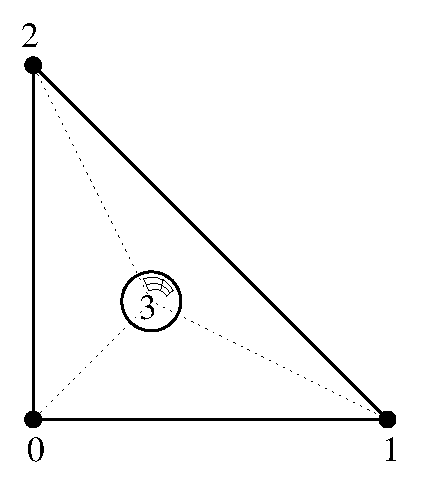
\includegraphics[width=5cm,angle=0]{getfemlist_triangle_P1_linbubble.eps}  \\
%       $P_1$ with additional bubble function, 4 d.o.f., $C^0$
%   \end{center}
%   \caption{ \it $P_1$ Lagrange element on a triangle with additional internal piecewise linear bubble function} 
%   \label{fig:triangle_p1_bubblepie}
% \end{figure}

% \begin{center}
% \begin{tabular}{|m{16.11cm}|} \hline 
% { \bf Lagrange $P_1$ with an additional internal piecewise linear bubble function}\\
% {\tt "FEM\_P1\_PIECEWISE\_LINEAR\_BUBBLE"} 
% \end{tabular} \\ \vspace{-1pt} 
% \begin{tabular}{|m{2cm}|m{2cm}|m{2.5cm}|m{1.2cm}|m{2cm}|m{2cm}|m{1.8cm}|} \hline 
% Degree & dimension & d.o.f. number & class & vectorial & \mbox{$\tau$-equivalent} & Polynomial\\ \hline
% $1$ & $2$ & $4$ & $C^0$ & No \mbox{($Q = 1$)} & Yes & No\\ \hline
% \end{tabular}
% \end{center}


% \begin{figure}[H]
%   \begin{center}
%     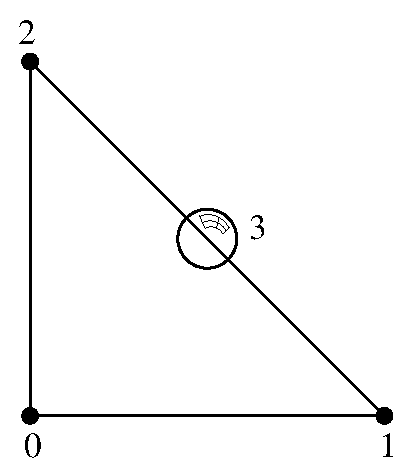
\includegraphics[width=5cm,angle=0]{getfemlist_triangle_P1_bubble_face.eps}
%   \end{center}
%   \caption{ \it $P_1$ Lagrange element on a triangle with additional bubble function on face 0, 4 d.o.f., $C^0$} 
%   \label{fig:triangle_p1_bubble_face}
% \end{figure}

% \begin{center}
% \begin{tabular}{|m{16.11cm}|} \hline 
% { \bf Lagrange $P_1$ element with an additional bubble function on face 0}\\
% {\tt "FEM\_P1\_BUBBLE\_FACE(2)"} 
% \end{tabular} \\ \vspace{-1pt} 
% \begin{tabular}{|m{2cm}|m{2cm}|m{2.5cm}|m{1.2cm}|m{2cm}|m{2cm}|m{1.8cm}|} \hline 
% Degree & dimension & d.o.f. number & class & vectorial & \mbox{$\tau$-equivalent} & Polynomial\\ \hline
% $2$ & $2$ & $4$ & $C^0$ & No \mbox{($Q = 1$)} & Yes & Yes\\ \hline
% \end{tabular}
% \end{center}

% \begin{figure}[H]
%   \begin{center}
%     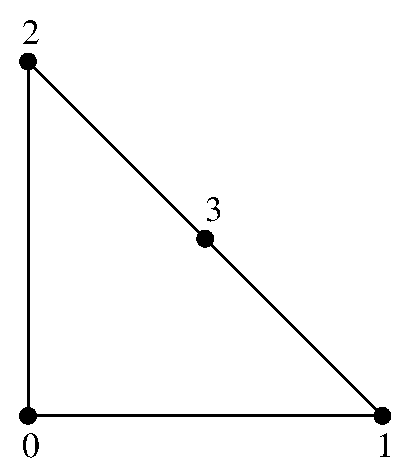
\includegraphics[width=5cm,angle=0]{getfemlist_triangle_P1_with_P2_face.eps}
%   \end{center}
%   \caption{ \it $P_1$ Lagrange element on a triangle with additional d.o.f on face 0, 4 d.o.f., $C^0$} 
%   \label{fig:triangle_p1_p2_face}
% \end{figure}

% \begin{center}
% \begin{tabular}{|m{16.11cm}|} \hline 
% { \bf $P_1$ Lagrange element on a triangle with additional d.o.f on face 0}\\
% {\tt "FEM\_P1\_BUBBLE\_FACE\_LAG"} 
% \end{tabular} \\ \vspace{-1pt} 
% \begin{tabular}{|m{2cm}|m{2cm}|m{2.5cm}|m{1.2cm}|m{2cm}|m{2cm}|m{1.8cm}|} \hline 
% Degree & dimension & d.o.f. number & class & vectorial & \mbox{$\tau$-equivalent} & Polynomial\\ \hline
% $2$ & $2$ & $4$ & $C^0$ & No \mbox{($Q = 1$)} & Yes & Yes\\ \hline
% \end{tabular}
% \end{center}

\subsubsection{Non-conforming $P_1$ element}


% \begin{figure}[H]
%   \begin{center}
%     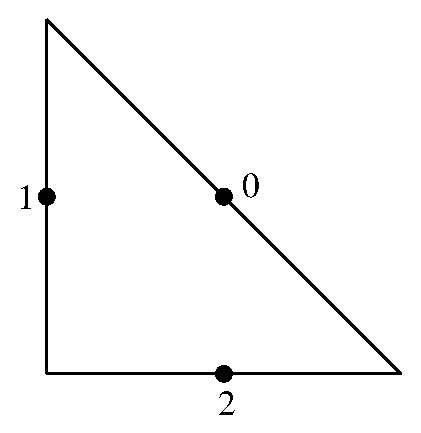
\includegraphics[width=5cm,angle=0]{getfemlist_triangle_P1_non_conforming.eps}
%   \end{center}
%   \caption{ \it $P_1$ non-conforming element on a triangle, 3 d.o.f., discontinuous} 
%   \label{fig:triangle_non_conforming}
% \end{figure}

% \begin{center}
% \begin{tabular}{|m{16.11cm}|} \hline 
% { \bf $P_1$ non-conforming element on a triangle}\\
% {\tt "FEM\_P1\_NONCONFORMING"} 
% \end{tabular} \\ \vspace{-1pt} 
% \begin{tabular}{|m{2cm}|m{2cm}|m{2.5cm}|m{1.2cm}|m{2cm}|m{2cm}|m{1.8cm}|} \hline 
% Degree & dimension & d.o.f. number & class & vectorial & \mbox{$\tau$-equivalent} & Polynomial\\ \hline
% $1$ & $2$ & $3$ & discon-tinuous & No \mbox{($Q = 1$)} & Yes & Yes\\ \hline
% \end{tabular}
% \end{center}

\subsubsection{Hermite element}

% \begin{figure}[H]
%   \begin{center}
%     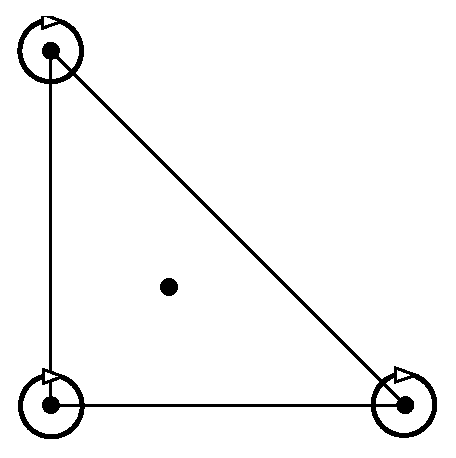
\includegraphics[width=6cm,angle=0]{getfemlist_triangle_hermite.eps}
%   \end{center}
%   \caption{ \it Hermite element on a triangle, $P_3$, 10 d.o.f., $C^0$ }
%   \label{fig:triangle_hermite}
% \end{figure}

Base functions on the reference element:
% $$
% \begin{array}{ll}
%   \varphi'_0 = (1-x-y)(1+x+y-2x^2-2y^2-11xy),~~ & (\varphi'_0(0,0) = 1), \\
%   \varphi'_1 = x(1-x-y)(1-x-2y), & (\partial_x\varphi'_1(0,0) = 1), \\
%   \varphi'_2 = y(1-x-y)(1-2x-y), & (\partial_y\varphi'_2(0,0) = 1), \\
%   \varphi'_3 = -2x^3 + 7 x^2y + 7xy^2 + 3x^2 - 7xy, & (\varphi'_3(1,0) = 1), \\
%   \varphi'_4 = x^3-2x^2y-2xy^2-x^2+2xy, & (\partial_x\varphi'_4(1,0) = 1), \\
%   \varphi'_5 = xy(y+2x-1), & (\partial_y\varphi'_5(1,0) = 1), \\
%   \varphi'_6 = 7x^2y + 7xy^2 - 2y^3+3y^2-7xy, & (\varphi'_6(0,1) = 1), \\
%   \varphi'_7 = xy(x+2y-1), & (\partial_x\varphi'_7(0,1) = 1), \\
%   \varphi'_8 = y^3-2x^2y-2xy^2-y^2+2xy, & (\partial_y\varphi'_8(0,1) = 1), \\
%   \varphi'_9 = 27xy(1-x-y), & (\varphi'_9(1/3,1/3) = 1), \\
% \end{array}
% $$
This element is not \mbox{$\tau$-equivalent} (The matrix $M$ is not equal to identity). On the real element linear combinaisons of $\varphi'_4$ and $\varphi'_7$ are used to match the gradient on the corresponding vertex. Idem for the two couples ($\varphi'_5$, $\varphi'_8$) and  ($\varphi'_6$, $\varphi'_9$) for the two other vertices.  

% \begin{center}
% \begin{tabular}{|m{16.11cm}|} \hline 
% { \bf Hermite element on a triangle}\\
% "FEM\_HERMITE(2)"
% \end{tabular} \\ \vspace{-1pt} 
% \begin{tabular}{|m{2cm}|m{2cm}|m{2.5cm}|m{1.2cm}|m{2cm}|m{2cm}|m{1.8cm}|} \hline 
% Degree & dimension & d.o.f. number & class & vectorial & \mbox{$\tau$-equivalent} & Polynomial\\ \hline
% $3$ & $2$ & $10$ & $C^0$ & No \mbox{($Q = 1$)} & No & Yes\\ \hline
% \end{tabular}
% \end{center}


\subsubsection{Morley element}

% \begin{figure}[H]
%   \begin{center}
%     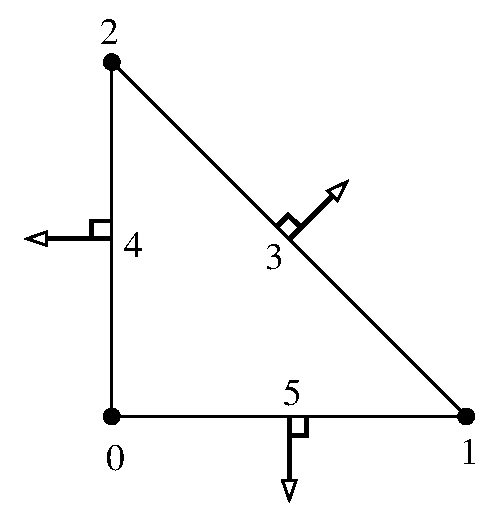
\includegraphics[width=6cm,angle=0]{getfemlist_morley.eps}
%   \end{center}
%   \caption{ \it tiangle Morley element, $P_2$, 6 d.o.f., $C^0$ }
%   \label{fig:triangle_morley}
% \end{figure}

This element is not \mbox{$\tau$-equivalent} (The matrix $M$ is not equal to identity). In particular, it can be used for non-conforming discretization of fourth order problems, despite the fact that it is not ${\cal C}^0$.

% \begin{center}
% \begin{tabular}{|m{16.11cm}|} \hline 
% { \bf Morley element on a triangle}\\
% "FEM\_MORLEY"
% \end{tabular} \\ \vspace{-1pt} 
% \begin{tabular}{|m{2cm}|m{2cm}|m{2.5cm}|m{1.2cm}|m{2cm}|m{2cm}|m{1.8cm}|} \hline 
% Degree & dimension & d.o.f. number & class & vectorial & \mbox{$\tau$-equivalent} & Polynomial\\ \hline
% $2$ & $2$ & $6$ &  & No \mbox{($Q = 1$)} & No & Yes\\ \hline
% \end{tabular}
% \end{center}

\subsubsection{Argyris element}

% \begin{figure}[H]
%   \begin{center}
%     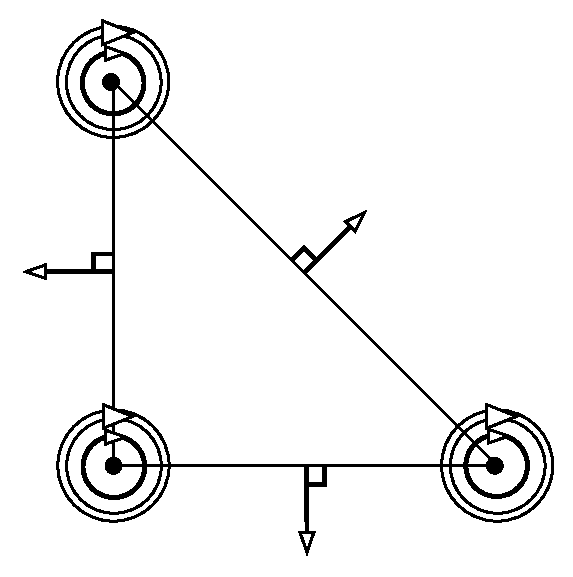
\includegraphics[width=6cm,angle=0]{getfemlist_argyris.eps}
%   \end{center}
%   \caption{ \it Argyris element, $P_5$, 21 d.o.f., $C^1$}
%   \label{fig:argyris}
% \end{figure}

% The base functions on the reference element are:
% $$ \begin{array}{ll}
% \varphi'_{0}(x,y) = 1 - 10x^3 - 10y^3 + 15x^4 - 30x^2y^2 + 15y^4 - 6x^5 + 30x^3y^2 + 30x^2y^3 - 6y^5, & (\varphi'_0(0,0) = 1), \\
% \varphi'_{1}(x,y) = x - 6x^3 - 11xy^2 + 8x^4 + 10x^2y^2 + 18xy^3 - 3x^5 + x^3y^2 - 10x^2y^3 - 8xy^4, & (\partial_x\varphi'_1(0,0) = 1),\\
% \varphi'_{2}(x,y) = y - 11x^2y - 6y^3 + 18x^3y + 10x^2y^2 + 8y^4 - 8x^4y - 10x^3y^2 + x^2y^3 - 3y^5, & (\partial_y\varphi'_2(0,0) = 1),\\
% \varphi'_{3}(x,y) = 0.5x^2 - 1.5x^3 + 1.5x^4 - 1.5x^2y^2 - 0.5x^5 + 1.5x^3y^2 + x^2y^3, & (\partial^2_{xx}\varphi'_3(0,0) = 1),\\
% \varphi'_{4}(x,y) = xy - 4x^2y - 4xy^2 + 5x^3y + 10x^2y^2 + 5xy^3 - 2x^4y - 6x^3y^2 - 6x^2y^3 - 2xy^4, & (\partial^2_{xy}\varphi'_{4}(0,0) = 1),\\
% \varphi'_{5}(x,y) = 0.5y^2 - 1.5y^3 - 1.5x^2y^2 + 1.5y^4 + x^3y^2 + 1.5x^2y^3 - 0.5y^5, & (\partial^2_{yy}\varphi'_{5}(0,0) = 1),\\
% \varphi'_{6}(x,y) = 10x^3 - 15x^4 + 15x^2y^2 + 6x^5 - 15x^3y^2 - 15x^2y^3, & (\varphi'_6(1,0) = 1),\\
% \varphi'_{7}(x,y) = -4x^3 + 7x^4 - 3.5x^2y^2 - 3x^5 + 3.5x^3y^2 + 3.5x^2y^3, & (\partial_x\varphi'_7(1,0) = 1),\\
% \varphi'_{8}(x,y) = -5x^2y + 14x^3y + 18.5x^2y^2 - 8x^4y - 18.5x^3y^2 - 13.5x^2y^3, & (\partial_y\varphi'_8(1,0) = 1),\\
% \varphi'_{9}(x,y) = 0.5x^3 - x^4 + 0.25x^2y^2 + 0.5x^5 - 0.25x^3y^2 - 0.25x^2y^3, & (\partial^2_{xx}\varphi'_{9}(1,0) = 1),\\
% \varphi'_{10}(x,y) = x^2y - 3x^3y - 3.5x^2y^2 + 2x^4y + 3.5x^3y^2 + 2.5x^2y^3, & (\partial^2_{xy}\varphi'_{10}(1,0) = 1),\\
% \varphi'_{11}(x,y) = 1.25x^2y^2 - 0.75x^3y^2 - 1.25x^2y^3, & (\partial^2_{yy}\varphi'_{11}(1,0) = 1),\\
% \varphi'_{12}(x,y) = 10y^3 + 15x^2y^2 - 15y^4 - 15x^3y^2 - 15x^2y^3 + 6y^5, & (\varphi'_{12}(0,1) = 1),\\
% \varphi'_{13}(x,y) = -5xy^2 + 18.5x^2y^2 + 14xy^3 - 13.5x^3y^2 - 18.5x^2y^3 - 8xy^4, & (\partial_x\varphi'_{13}(0,1) = 1),\\
% \varphi'_{14}(x,y) = -4y^3 - 3.5x^2y^2 + 7y^4 + 3.5x^3y^2 + 3.5x^2y^3 - 3y^5, & (\partial_y\varphi'_{14}(0,0) = 1),\\
% \varphi'_{15}(x,y) = 1.25x^2y^2 - 1.25x^3y^2 - 0.75x^2y^3, & (\partial^2_{xx}\varphi'_{15}(0,1) = 1),\\
% \varphi'_{16}(x,y) = xy^2 - 3.5x^2y^2 - 3xy^3 + 2.5x^3y^2 + 3.5x^2y^3 + 2xy^4, & (\partial^2_{xy}\varphi'_{16}(0,1) = 1),\\
% \varphi'_{17}(x,y) = 0.5y^3 + 0.25x^2y^2 - y^4 - 0.25x^3y^2 - 0.25x^2y^3 + 0.5y^5, & (\partial^2_{yy}\varphi'_{17}(0,1) = 1),\\
% \varphi'_{18}(x,y) = \sqrt{2}(-8x^2y^2 + 8x^3y^2 + 8x^2y^3), & \hspace*{-9.5em}(\sqrt{0.5}(\partial_{x}\varphi'_{18}(0.5,0.5) + \partial_{y}\varphi'_{18}(0.5,0.5)) = 1),\\
% \varphi'_{19}(x,y) = -16xy^2 + 32x^2y^2 + 32xy^3 - 16x^3y^2 - 32x^2y^3 - 16xy^4, & (-\partial_{x}\varphi'_{19}(0,0.5) = 1),\\
% \varphi'_{20}(x,y) = -16x^2y + 32x^3y + 32x^2y^2 - 16x^4y - 32x^3y^2 - 16x^2y^3, & (-\partial_{y}\varphi'_{20}(0.5,0) = 1),\\
% \end{array}
% $$

This element is not \mbox{$\tau$-equivalent} (The matrix $M$ is not equal to identity). On the real element linear combinaisons of the transformed base functions $\varphi'_i$ are used to match the gradient, the second derivatives and the normal derivatives on the faces. Note that the use of the matrix  $M$ (see also the documentation on the finite element kernel \cite{BAS_COMP}) allows to define Argyris element even with nonlinear geometric transformations (for instance to treat curved boundaries).


% \begin{center}
% \begin{tabular}{|m{16.11cm}|} \hline 
% { \bf Argyris element on a triangle}\\
% "FEM\_ARGYRIS"
% \end{tabular} \\ \vspace{-1pt}
% \begin{tabular}{|m{2cm}|m{2cm}|m{2.5cm}|m{1.2cm}|m{2cm}|m{2cm}|m{1.8cm}|} \hline 
% Degree & dimension & d.o.f. number & class & vectorial & \mbox{$\tau$-equivalent} & Polynomial\\ \hline
% $5$ & $2$ & $21$ & $C^1$ & No \mbox{($Q = 1$)} & No & Yes\\ \hline
% \end{tabular}
% \end{center}

\subsubsection{Hsieh-Clough-Tocher element}

% \begin{figure}[H]
%   \begin{center}
%     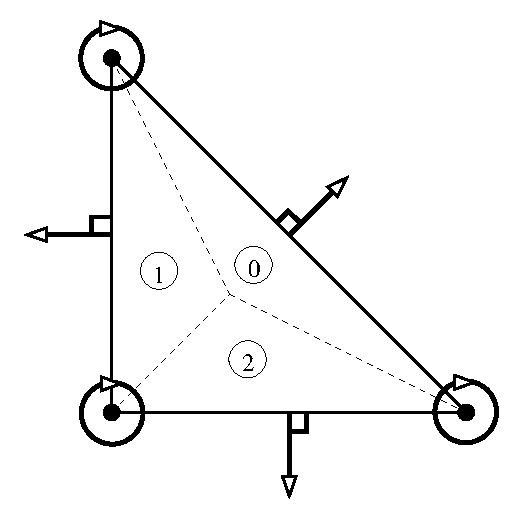
\includegraphics[width=6cm,angle=0]{getfemlist_HCT.eps}
%   \end{center}
%   \caption{ \it Hsieh-Clough-Tocher (HCT) element, $P_3$, 12 d.o.f., $C^1$}
%   \label{fig:HCT_tr}
% \end{figure}

This element is not \mbox{$\tau$-equivalent}. This is a composite element. Polynomial of degree 3 on each of the three sub-triangles (see figure \ref{fig:HCT_tr} and \cite{ciarlet1978}). It is strongly advised to use a \cpp{ IM\_HCT\_COMPOSITE } integration method with this finite element. The numeration of the dof is the following : 0, 3 and 6 for the lagrange dof on the first second and third vertex respectively; 1, 4, 7 for the derivative with respects to the first variable; 2, 5, 8 for the derivative with respects to the second variable and 9, 10, 11 for the normal derivatives on face 0, 1, 2 respectively.\\

% \begin{center}
% \begin{tabular}{|m{16.11cm}|} \hline 
% { \bf HCT element on a triangle}\\
% "FEM\_HCT\_TRIANGLE"
% \end{tabular} \\ \vspace{-1pt} 
% \begin{tabular}{|m{2cm}|m{2cm}|m{2.5cm}|m{1.2cm}|m{2cm}|m{2cm}|m{1.8cm}|} \hline 
% Degree & dimension & d.o.f. number & class & vectorial & \mbox{$\tau$-equivalent} & Polynomial \\ \hline
% $3$ & $2$ & $12$ & $C^1$ & No \mbox{($Q = 1$)} & No & composite\\ \hline
% \end{tabular}
% \end{center}


% \begin{figure}[H]
%   \begin{center}
%     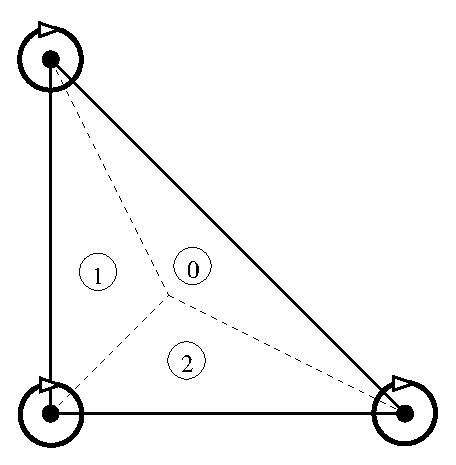
\includegraphics[width=5.5cm,angle=0]{getfemlist_reduced_HCT.eps}
%   \end{center}
%   \caption{ \it Reduced Hsieh-Clough-Tocher (reduced HCT) element, $P_3$, 9 d.o.f., $C^1$}
%   \label{fig:reduced_HCT_tr}
% \end{figure}

% This element exists also in its reduced form, where the normal derivatives is assumed to be polynomial of degree one on each edge (see figure \ref{fig:reduced_HCT_tr})



% \begin{center}
% \begin{tabular}{|m{16.11cm}|} \hline 
% { \bf Reduced HCT element on a triangle}\\
% "FEM\_REDUCED\_HCT\_TRIANGLE"
% \end{tabular} \\ \vspace{-1pt} 
% \begin{tabular}{|m{2cm}|m{2cm}|m{2.5cm}|m{1.2cm}|m{2cm}|m{2cm}|m{1.8cm}|} \hline 
% Degree & dimension & d.o.f. number & class & vectorial & \mbox{$\tau$-equivalent} & Polynomial \\ \hline
% $3$ & $2$ & $9$ & $C^1$ & No \mbox{($Q = 1$)} & No & composite\\ \hline
% \end{tabular}
% \end{center}

\subsubsection{A composite $C^1$ element on quadrilaterals}

% \begin{figure}[H]
%   \begin{center}
%     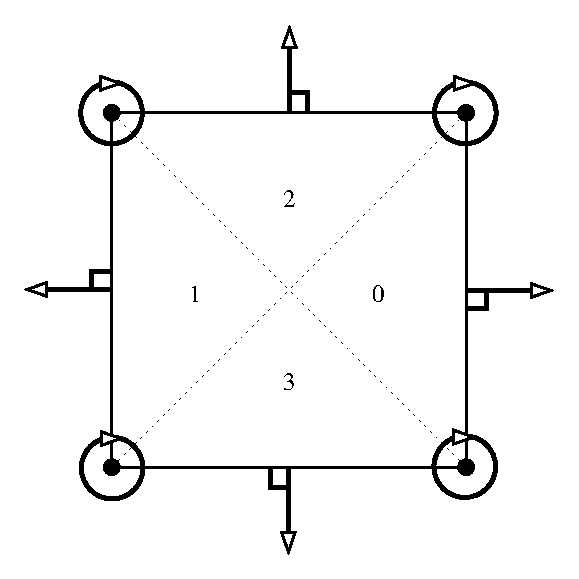
\includegraphics[width=6cm,angle=0]{getfemlist_quadc1_composite.eps}
%   \end{center}
%   \caption{ \it Composite element on quadrilaterals, piecewise $P_3$, 16 d.o.f., $C^1$}
%   \label{fig:QC1_tr}
% \end{figure}

This element is not \mbox{$\tau$-equivalent}. This is a composite element. Polynomial of degree 3 on each of the four sub-triangles (see figure \ref{fig:QC1_tr}). At least on the reference element it correponds to the Fraeijs de Veubeke-Sander element (see \cite{ciarlet1978}). It is strongly advised to use a \cpp{ IM\_QUADC1\_COMPOSITE } integration method with this finite element. \\

% \begin{center}
% \begin{tabular}{|m{16.11cm}|} \hline 
% { \bf HCT element on a triangle}\\
% "FEM\_QUADC1\_COMPOSITE"
% \end{tabular} \\ \vspace{-1pt} 
% \begin{tabular}{|m{2cm}|m{2cm}|m{2.5cm}|m{1.2cm}|m{2cm}|m{2cm}|m{1.8cm}|} \hline 
% Degree & dimension & d.o.f. number & class & vectorial & \mbox{$\tau$-equivalent} & Polynomial \\ \hline
% $3$ & $2$ & $16$ & $C^1$ & No \mbox{($Q = 1$)} & No & composite\\ \hline
% \end{tabular}
% \end{center}


% \begin{figure}[H]
%   \begin{center}
%     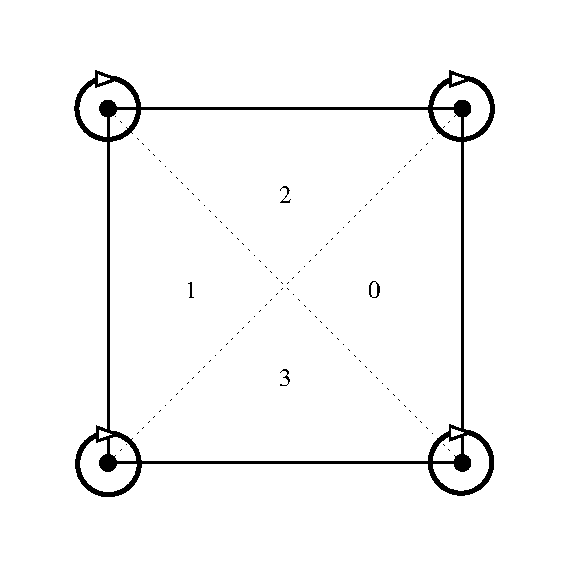
\includegraphics[width=5.5cm,angle=0]{getfemlist_reduced_quadc1_composite.eps}
%   \end{center}
%   \caption{ \it Reduced composite element on quadrilaterals, piecewise $P_3$, 12 d.o.f., $C^1$}
%   \label{fig:reduced_QC1_tr}
% \end{figure}

This element exists also in its reduced form, where the normal derivatives is assumed to be polynomial of degree one on each edge (see figure \ref{fig:reduced_QC1_tr})


% \begin{center}
% \begin{tabular}{|m{16.11cm}|} \hline 
% { \bf Reduced HCT element on a triangle}\\
% "FEM\_REDUCED\_QUADC1\_COMPOSITE"
% \end{tabular} \\ \vspace{-1pt} 
% \begin{tabular}{|m{2cm}|m{2cm}|m{2.5cm}|m{1.2cm}|m{2cm}|m{2cm}|m{1.8cm}|} \hline 
% Degree & dimension & d.o.f. number & class & vectorial & \mbox{$\tau$-equivalent} & Polynomial \\ \hline
% $3$ & $2$ & $12$ & $C^1$ & No \mbox{($Q = 1$)} & No & composite\\ \hline
% \end{tabular}
% \end{center}





\subsection{Specific elements in dimension 3}
\subsubsection{Elements with additional bubble functions}
% \begin{figure}[H]
%   \begin{center}
%     \begin{tabular}{m{5cm}m{5cm}m{5cm}}
%       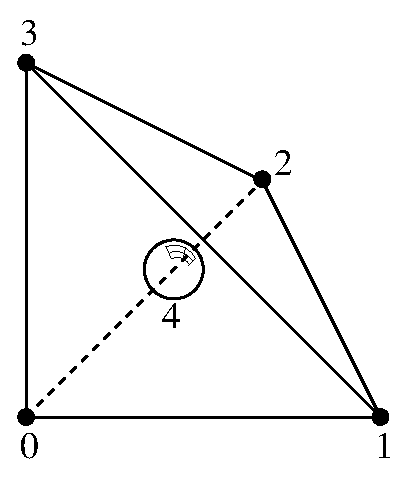
\includegraphics[width=4.5cm,angle=0]{getfemlist_tetrahedron_P1_bubble.eps} & 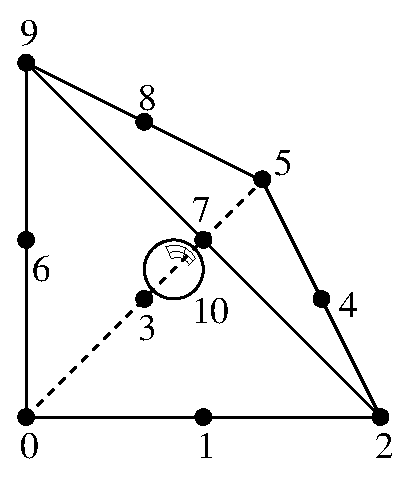
\includegraphics[width=4.5cm,angle=0]{getfemlist_tetrahedron_P2_bubble.eps} & 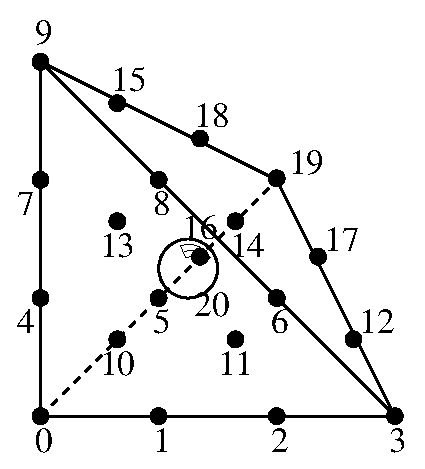
\includegraphics[width=4.5cm,angle=0]{getfemlist_tetrahedron_P3_bubble.eps}  \\
%       $P_1$ with additional bubble function, 5 d.o.f., $C^0$ & $P_2$ with additional bubble function, 11 d.o.f., $C^0$ & $P_3$ with additional bubble function, 21 d.o.f., $C^0$
%     \end{tabular}
%   \end{center}
%   \caption{ \it Lagrange element on a tetrahedron with additional internal bubble function.} 
%   \label{fig:tetrahedron_p1_bubble}
% \end{figure}

% \begin{center}
% \begin{tabular}{|m{16.11cm}|} \hline 
% { \bf $P_K$ Lagrange element with an additional internal bubble function}\\
% {\tt "FEM\_PK\_WITH\_CUBIC\_BUBBLE(3, K)"} 
% \end{tabular} \\ \vspace{-1pt} 
% \begin{tabular}{|m{2cm}|m{2cm}|m{2.5cm}|m{1.2cm}|m{2cm}|m{2cm}|m{1.8cm}|} \hline 
% Degree & dimension & d.o.f. number & class & vectorial & \mbox{$\tau$-equivalent} & Polynomial\\ \hline
% $4$ & $3$ & $5$, $11$ or $21$ & $C^0$ & No \mbox{($Q = 1$)} & Yes & Yes\\ \hline
% \end{tabular}
% \end{center}

% \begin{figure}[H]
%   \begin{center}
%     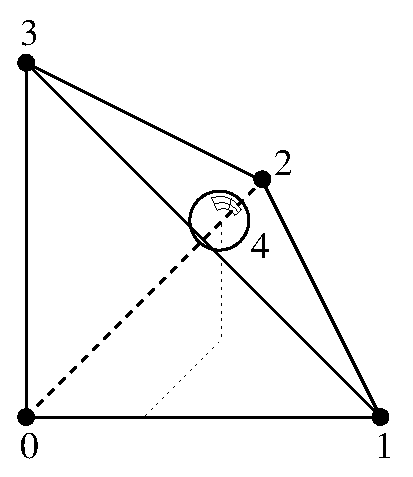
\includegraphics[width=5cm,angle=0]{getfemlist_tetrahedron_P1_bubble_face.eps}
%   \end{center}
%   \caption{ \it $P_1$ Lagrange element on a tetrahedron with additional bubble function on face 0, 5 d.o.f., $C^0$} 
%   \label{fig:tetrahedron_p1_bubble_face}
% \end{figure}

% \begin{center}
% \begin{tabular}{|m{16.11cm}|} \hline 
% { \bf Lagrange $P_1$ element with an additional bubble function on face 0}\\
% {\tt "FEM\_P1\_BUBBLE\_FACE(3)"} 
% \end{tabular} \\ \vspace{-1pt} 
% \begin{tabular}{|m{2cm}|m{2cm}|m{2.5cm}|m{1.2cm}|m{2cm}|m{2cm}|m{1.8cm}|} \hline 
% Degree & dimension & d.o.f. number & class & vectorial & \mbox{$\tau$-equivalent} & Polynomial\\ \hline
% $3$ & $3$ & $5$ & $C^0$ & No \mbox{($Q = 1$)} & Yes & Yes\\ \hline
% \end{tabular}
% \end{center}

\subsubsection{Hermite element}

% \begin{figure}[H]
%   \begin{center}
%     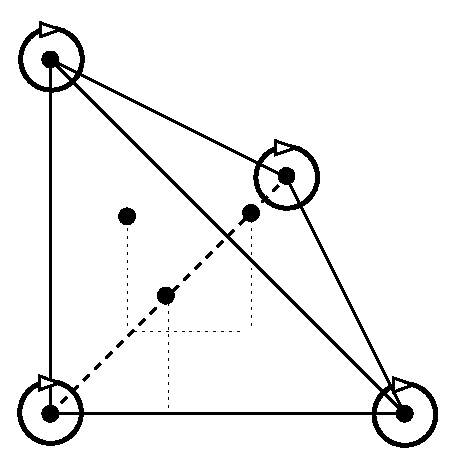
\includegraphics[width=6cm,angle=0]{getfemlist_tetrahedron_hermite.eps}
%   \end{center}
%   \caption{ \it Hermite element on a tetrahedron, $P_3$, 20 d.o.f., $C^0$}
%   \label{fig:tetrahedron_hermite}
% \end{figure}

Base functions on the reference element:
% $$
%   \begin{array}{ll}
% \varphi'_{0}(x,y) = 1 - 3x^2 - 13xy - 13xz - 3y^2 - 13yz - 3z^2 + 2x^3 + 13x^2y + 13x^2z & \\
%  ~~~~~~~~~~~~~~~ + 13xy^2 + 33xyz + 13xz^2 + 2y^3 + 13y^2z + 13yz^2 + 2z^3, & (\varphi'_0(0,0,0) = 1),\\
% \varphi'_{1}(x,y) = x - 2x^2 - 3xy - 3xz + x^3 + 3x^2y + 3x^2z + 2xy^2 + 4xyz + 2xz^2, & (\partial_x\varphi'_1(0,0,0) = 1),\\
% \varphi'_{2}(x,y) = y - 3xy - 2y^2 - 3yz + 2x^2y + 3xy^2 + 4xyz + y^3 + 3y^2z + 2yz^2, & (\partial_y\varphi'_2(0,0,0) = 1),\\
% \varphi'_{3}(x,y) = z - 3xz - 3yz - 2z^2 + 2x^2z + 4xyz + 3xz^2 + 2y^2z + 3yz^2 + z^3, & (\partial_z\varphi'_3(0,0,0) = 1),\\
% \varphi'_{4}(x,y) = 3x^2 - 7xy - 7xz - 2x^3 + 7x^2y + 7x^2z + 7xy^2 + 7xyz + 7xz^2, & (\varphi'_4(1,0,0) = 1),\\
% \varphi'_{5}(x,y) = -x^2 + 2xy + 2xz + x^3 - 2x^2y - 2x^2z - 2xy^2 - 2xyz - 2xz^2, & (\partial_x\varphi'_5(1,0,0) = 1),\\
% \varphi'_{6}(x,y) = -xy + 2x^2y + xy^2, & (\partial_y\varphi'_6(1,0,0) = 1),\\
% \varphi'_{7}(x,y) = -xz + 2x^2z + xz^2, & (\partial_z\varphi'_7(1,0,0) = 1),\\
% \varphi'_{8}(x,y) = -7xy + 3y^2 - 7yz + 7x^2y + 7xy^2 + 7xyz - 2y^3 + 7y^2z + 7yz^2, & (\varphi'_8(0,1,0) = 1),\\
% \varphi'_{9}(x,y) = -xy + x^2y + 2xy^2, & (\partial_x\varphi'_9(0,1,0) = 1),\\
% \varphi'_{10}(x,y) = 2xy - y^2 + 2yz - 2x^2y - 2xy^2 - 2xyz + y^3 - 2y^2z - 2yz^2, & (\partial_y\varphi'_{10}(0,1,0) = 1),\\
% \varphi'_{11}(x,y) = -yz + 2y^2z + yz^2, & (\partial_z\varphi'_{11}(0,1,0) = 1),\\
% \varphi'_{12}(x,y) = -7xz - 7yz + 3z^2 + 7x^2z + 7xyz + 7xz^2 + 7y^2z + 7yz^2 - 2z^3, & (\varphi'_{12}(0,0,1) = 1),\\
% \varphi'_{13}(x,y) = -xz + x^2z + 2xz^2, & (\partial_x\varphi'_{13}(0,0,1) = 1),\\
% \varphi'_{14}(x,y) = -yz + y^2z + 2yz^2, & (\partial_y\varphi'_{14}(0,0,1) = 1),\\
% \varphi'_{15}(x,y) = 2xz + 2yz - z^2 - 2x^2z - 2xyz - 2xz^2 - 2y^2z - 2yz^2 + z^3, & (\partial_z\varphi'_{15}(0,0,1) = 1),\\
% \varphi'_{16}(x,y) = 27xyz, & (\varphi'_{16}(1/3,1/3,1/3) = 1),\\
% \varphi'_{17}(x,y) = 27yz - 27xyz - 27y^2z - 27yz^2, & (\varphi'_{17}(0,1/3,1/3) = 1),\\
% \varphi'_{18}(x,y) = 27xz - 27x^2z - 27xyz - 27xz^2, & (\varphi'_{18}(1/3,0,1/3) = 1),\\
% \varphi'_{19}(x,y) = 27xy - 27x^2y - 27xy^2 - 27xyz, & (\varphi'_{19}(1/3,1/3,0) = 1),\\

%   \end{array}
% $$
This element is not \mbox{$\tau$-equivalent} (The matrix $M$ is not equal to identity). On the real element linear combinaisons of $\varphi'_8$, $\varphi'_{12}$ and $\varphi'_{16}$ are used to match the gradient on the corresponding vertex. Idem on the orther vertices. 

% \begin{center}
% \begin{tabular}{|m{16.11cm}|} \hline 
% { \bf Hermite element on a tetrahedron}\\
% "FEM\_HERMITE(3)"
% \end{tabular} \\ \vspace{-1pt} 
% \begin{tabular}{|m{2cm}|m{2cm}|m{2.5cm}|m{1.2cm}|m{2cm}|m{2cm}|m{1.8cm}|} \hline 
% Degree & dimension & d.o.f. number & class & vectorial & \mbox{$\tau$-equivalent} & Polynomial\\ \hline
% $3$ & $3$ & $20$ & $C^0$ & No \mbox{($Q = 1$)} & No & Yes\\ \hline
% \end{tabular}
% \end{center}

\subsection{Interpolation of elements on different meshes}

% \begin{figure}[H]
%   \begin{center}
%     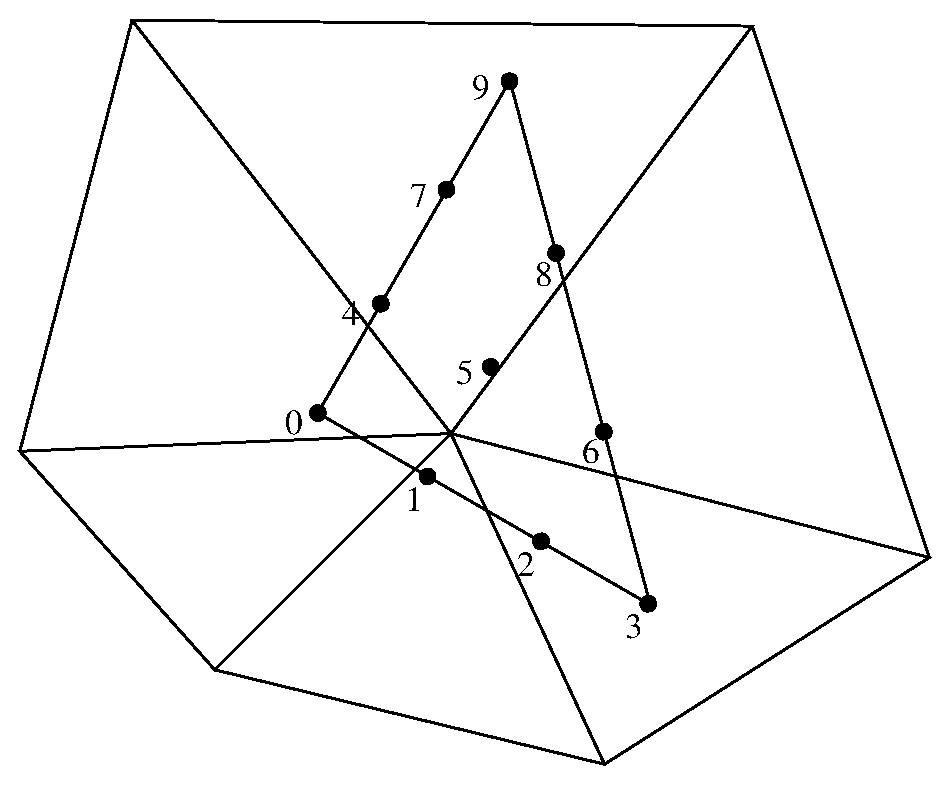
\includegraphics[width=5cm,angle=0]{getfemlist_virtual_fem.eps}
%   \end{center}
%   \caption{ \it Element which intepolates a finite element method defined on another mesh. The element has as many d.o.f. as the union of d.o.f. of elements of the other mesh having an intersection with it. The interpolation is made on Gauss points of the integration method.} 
%   \label{fig:virtual_fem}
% \end{figure}

To increase the precision, it is not necessary to raise the order of the integration method. It is recommended to keep the normal order and use composite integration methods (see below).

% \begin{center}
% \begin{tabular}{|m{16.11cm}|} \hline 
% { \bf Element which interpolates an element defined on another mesh}\\
%   {\tt getfem::virtual\_link\_fem(getfem::mesh\_fem mf1, getfem::mesh\_fem mf2,} \\ {\tt \mbox{}\hspace{12em} getfem::pintegration\_method pim) } \\
%   {\tt \mbox{}\hspace{5em} getfem::virtual\_link\_fem\_with\_gradient(getfem::mesh\_fem mf1, } \\ {\tt \hspace{5em} getfem::mesh\_fem mf2, \mbox{}getfem::pintegration\_method pim) } \\  \hline 
% \end{tabular} \\ \vspace{-1pt} 
% \end{center}





\section{Appendix B. Cubature method list}



% \subsection{Integration methods description}

% The integration methods are of two kinds. Exact integrations of polynomials and approximated integrations (cubature formulas) of any function. The exact integration can only be used if all the elements are polynomial and if the geometric transformation is linear.

%  A descriptor on an integration method is available thanks to the function\\[0.5cm]
% {\tt
%   ppi = getfem::int\_method\_descriptor("name of method");
% }\\[0.5cm]
% where {\tt "name of method"} is a string to be choosen among the existing methods.

% The program \cpp{integration} located in the \cpp{tests} directory lists and checks the degree of each integration method.

% \subsection{Exact Integration methods}

% The list of available Exact integration methods is the following

% \begin{center} \begin{tabular}{|m{0.55\linewidth}|m{0.4\linewidth}|} \hline
{\tt "IM\_EXACT\_SIMPLEX(n)"} & Description of the exact integration of polynomials on the simplex of reference of dimension {\tt n}. \\ \hline
\end{tabular}  
\begin{tabular}{|m{0.55\linewidth}|m{0.4\linewidth}|} \hline
{\tt "IM\_PRODUCT(a, b)"} & Description of the exact integration on the convex which is the direct product of the convex in {\tt a} and in {\tt b}.\\ \hline
\end{tabular}  
\begin{tabular}{|m{0.55\linewidth}|m{0.4\linewidth}|} \hline
{\tt "IM\_EXACT\_PARALLELEPIPED(n)"} & Description of the exact integration of polynomials on the parallelepiped of reference of dimension {\tt n}\\ \hline
\end{tabular}  
\begin{tabular}{|m{0.55\linewidth}|m{0.4\linewidth}|} \hline
{\tt "IM\_EXACT\_PRISM(n)"} & Description of the exact integration of polynomials on the prism of reference of dimension {\tt n}\\ \hline
\end{tabular} \end{center}


% Even though a description of exact integration method exists on parallelepipeds or prisms, most of the time the geometric transformations on such elements are not linear and the exact integration cannot be used.\\

% Beware : In fact a lot of computation cannot be done with exact integration methods. So, it is recommended to use cubature formulas instead.

% \subsection{Newton cotes Integration methods}

% use {\tt "IM\_NC(N,K)"}, {\tt "IM\_NC\_PARALLELEPIPED(N,K)"}
% and {\tt "IM\_NC\_PRISM(N,K)"} to have the Newton cotes integration of order {\tt K} respectively on simplices, parallelepipeds and prisms.


% \subsection{Gauss Integration methods on dimension 1}

% use {\tt "IM\_GAUSS1D(K)"} to have the Gauss-Legendre integration on the segment of order {\tt K} (with {\tt K}/2 + 1 points), and {\tt "IM\_GAUSSLOBATTO1D(K)"} to have the Gauss-Lobatto-Legendre integration on the segment of order {\tt K} (with {\tt K}/2 + 1 points). The latter integration method is only available for odd values of $K$. The Gauss-Lobatto integration method can be used in conjunction with {\tt "FEM\_PK\_GAUSSLOBATTO1D(K/2)"} to perform mass-lumping.

% \subsection{Gauss Integration methods on dimension 2}

% \begin{tabular}{|m{2.5cm}|m{6cm}|m{1.2cm}|m{6.5cm}|} \hline 
% graphic & coordinates \hspace{5em} \begin{tabular}{m{3cm}m{3cm}} x & y  \end{tabular} & weights & function to call / order \\ \hline
% \end{tabular}
% \begin{tabular}{|m{2.5cm}|m{6cm}|m{1.2cm}|m{6.5cm}|}
%   \hline& & &\\ 
%   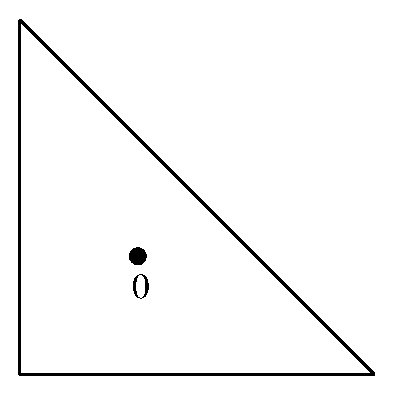
\includegraphics[width=2.5cm,angle=0]{getfemlist_intmethod_triangle1.eps} & 
%   { \small
%     \begin{tabular}{m{3cm}m{3cm}}
%       $1/3$ & $1/3$ 
%     \end{tabular}
%     }
%   & 
%     \begin{tabular}{c}
%       1/2
%     \end{tabular}
%   & {\tt \small "IM\_TRIANGLE(1)"} \hspace{9em} 
%     1 point, order 1. \\ \hline
% \end{tabular}
% \begin{tabular}{|m{2.5cm}|m{6cm}|m{1.2cm}|m{6.5cm}|}
%   \hline& & &\\ 
%   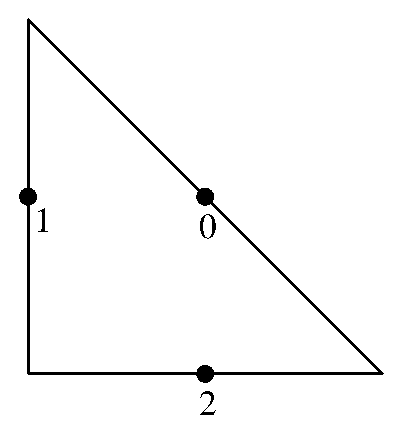
\includegraphics[width=2.5cm,angle=0]{getfemlist_intmethod_triangle2.eps} & 
%   { \small
%     \begin{tabular}{m{3cm}m{3cm}}
%       $1/6$ & $1/6$ \\ \\
%       $2/3$ & $1/6$  \\ \\
%       $1/6$ & $2/3$
%     \end{tabular}
%     }
%   & 
%     \begin{tabular}{c}
%       1/6 \\ \\
%       1/6 \\ \\
%       1/6
%     \end{tabular}
%   & {\tt \small "IM\_TRIANGLE(2)"} \hspace{9em} 3 points, order 2. \\ \hline
% \end{tabular} 
% \begin{tabular}{|m{2.5cm}|m{6cm}|m{1.2cm}|m{6.5cm}|}
%   \hline& & &\\ 
%   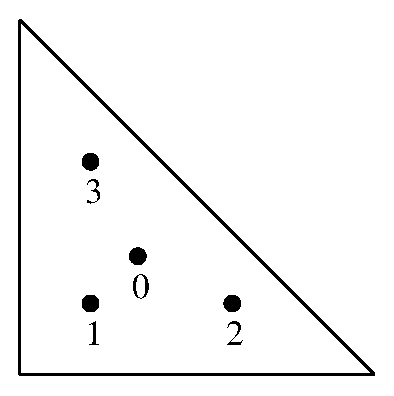
\includegraphics[width=2.5cm,angle=0]{getfemlist_intmethod_triangle3.eps} & 
%   { \small
%     \begin{tabular}{m{3cm}m{3cm}}
%       $1/3$ & $1/3$ \\ \\
%       $1/5$ & $1/5$ \\ \\
%       $3/5$ & $1/5$ \\ \\
%       $1/5$ & $3/5$
%     \end{tabular}
%     }
%   & { \small
%     \begin{tabular}{c}
%       -27/96 \\ \\
%       25/96 \\ \\
%       25/96 \\ \\ 
%       25/96 
%     \end{tabular} }
%   & {\tt \small "IM\_TRIANGLE(3)"} \hspace{9em} 4 points, order 3. \\ \hline
% \end{tabular} 
% \begin{tabular}{|m{2.5cm}|m{6cm}|m{1.2cm}|m{6.5cm}|}
%   \hline& & &\\ 
%   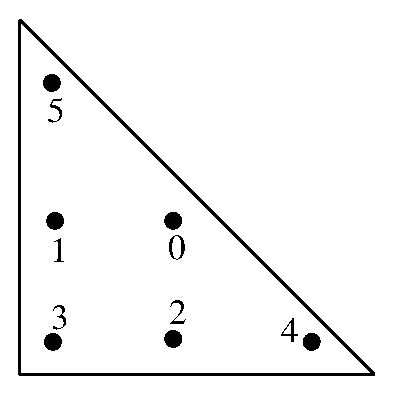
\includegraphics[width=2.5cm,angle=0]{getfemlist_intmethod_triangle4.eps} & 
%   { \small
%     \begin{tabular}{m{3cm}m{3cm}}
%       $a$ & $a$ \\ 
%       $1-2a$ & $a$ \\ 
%       $a$ & $1-2a$ \\ 
%       $b$ & $b$ \\ 
%       $1-2b$ & $b$  \\ 
%       $b$ & $1-2b$
%     \end{tabular}
%     }
%   & { \small
%     \begin{tabular}{c}
%       c \\ 
%       c \\ 
%       c \\ 
%       d \\ 
%       d \\ 
%       d
%     \end{tabular} }
%   & {\tt \small "IM\_TRIANGLE(4)"} \hspace{7em} \mbox{6 points, order 4,}\hspace{7em} \mbox{a = 0.445948490915965,}\hspace{5em} \mbox{b = 0.091576213509771,}\hspace{5em} \mbox{c = 0.111690794839005,}\hspace{5em} \mbox{d = 0.054975871827661.} \\ \hline
% \end{tabular} 
% \begin{tabular}{|m{2.5cm}|m{6cm}|m{1.2cm}|m{6.5cm}|}
%   \hline& & &\\ 
%   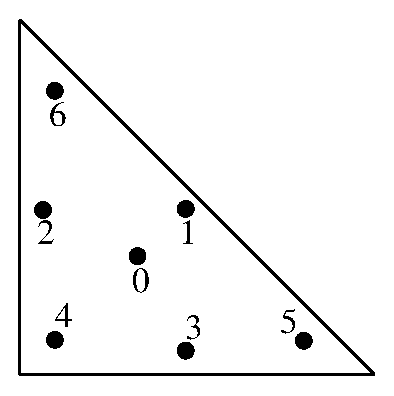
\includegraphics[width=2.5cm,angle=0]{getfemlist_intmethod_triangle5.eps} & 
%   { \small
%     \begin{tabular}{m{3cm}m{3cm}}
%       $1/3$ & $1/3$ \\ 
%       $a$ & $a$ \\ 
%       $1-2a$ & $a$ \\ 
%       $a$ & $1-2a$ \\ 
%       $b$ & $b$ \\ 
%       $1-2b$ & $b$  \\ 
%       $b$ & $1-2b$
%     \end{tabular}
%     }
%   & { \small
%     \begin{tabular}{c}
%       9/80 \\ 
%       c \\ 
%       c \\ 
%       c \\ 
%       d \\ 
%       d \\ 
%       d 
%     \end{tabular} }
%   & {\tt \small "IM\_TRIANGLE(5)"} \hspace{7em} \mbox{7 points, order 5,}\hspace{7em} \mbox{$a = \Frac{6+\sqrt{15}}{21}$,}\hspace{5em} \mbox{$b = 4/7 - a$,}\hspace{8em} \mbox{$c = \Frac{155+\sqrt{15}}{2400}$,}\hspace{5em} \mbox{$d = 31/240 - c$.} \\ \hline
% \end{tabular}  
% \begin{tabular}{|m{2.5cm}|m{6cm}|m{1.2cm}|m{6.5cm}|}
%   \hline& & &\\ 
%   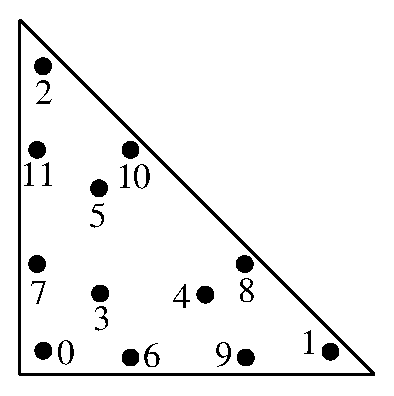
\includegraphics[width=2.5cm,angle=0]{getfemlist_intmethod_triangle6.eps} & 
%   { \small
%     \begin{tabular}{m{3cm}m{3cm}}
%       $a$ & $a$ \\ 
%       $1-2a$ & $a$ \\ 
%       $a$ & $1-2a$ \\ 
%       $b$ & $b$ \\ 
%       $1-2b$ & $b$ \\ 
%       $b$ & $1-2b$ \\ 
%       $c$ & $d$ \\ 
%       $d$ & $c$ \\ 
%       $1-c-d$ & $c$ \\ 
%       $1-c-d$ & $d$ \\ 
%       $c$ & $1-c-d$ \\ 
%       $d$ & $1-c-d$
%     \end{tabular}
%     }
%   & { \small
%     \begin{tabular}{c}
%       e \\
%       e \\ 
%       e \\ 
%       f \\  
%       f \\ 
%       f \\ 
%       g \\ 
%       g \\ 
%       g \\ 
%       g \\ 
%       g \\ 
%       g
%     \end{tabular} }
%   & {\tt \small "IM\_TRIANGLE(6)"} \hspace{7em} \mbox{12 points, order 6,}\hspace{7em}
%   \mbox{$a = 0.063089104491502$,}\hspace{5em}
%   \mbox{$b = 0.249286745170910$,}\hspace{8em}
%   \mbox{$c = 0.310352451033785$,}\hspace{5em}
%   \mbox{$d = 0.053145049844816$,}\hspace{5em}
%   \mbox{$e = 0.025422453185103$,}\hspace{5em}
%   \mbox{$f = 0.058393137863189$,}\hspace{5em}
%   \mbox{$g = 0.041425537809187$.}\hspace{5em}
%   \\ \hline
% \end{tabular}  
% \begin{tabular}{|m{2.5cm}|m{6cm}|m{1.2cm}|m{6.5cm}|}
%   \hline& & &\\ 
%   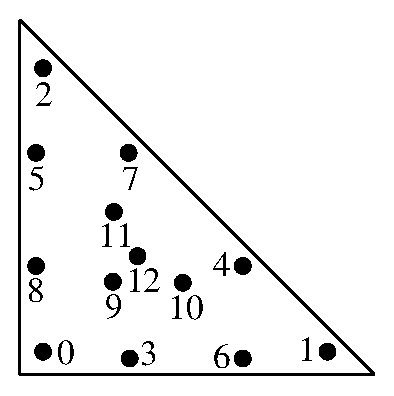
\includegraphics[width=2.5cm,angle=0]{getfemlist_intmethod_triangle7.eps} & 
%   { \small
%     \begin{tabular}{m{3cm}m{3cm}}
%       $a$ & $a$ \\ 
%       $b$ & $a$ \\ 
%       $a$ & $b$ \\ 
%       $c$ & $e$ \\ 
%       $d$ & $c$ \\ 
%       $e$ & $d$ \\ 
%       $d$ & $e$ \\ 
%       $c$ & $d$ \\ 
%       $e$ & $c$ \\ 
%       $f$ & $f$ \\ 
%       $g$ & $f$ \\ 
%       $f$ & $g$ \\
%       $1/3$ & $1/3$ 
%     \end{tabular}
%     }
%   & { \small
%     \begin{tabular}{c}
%       h \\
%       h \\ 
%       h \\ 
%       i \\  
%       i \\ 
%       i \\ 
%       i \\ 
%       i \\ 
%       i \\
%       j \\
%       j \\
%       j \\
%       k
%     \end{tabular} }
%   & {\tt \small "IM\_TRIANGLE(7)"} \hspace{7em} \mbox{13 points, order 7,}\hspace{7em}
%   \mbox{$a = 0.0651301029022$,}\hspace{5em}
%   \mbox{$b = 0.8697397941956$,}\hspace{5em}
%   \mbox{$c = 0.3128654960049$,}\hspace{5em}
%   \mbox{$d = 0.6384441885698$,}\hspace{5em}
%   \mbox{$e = 0.0486903154253$,}\hspace{5em}
%   \mbox{$f = 0.2603459660790$,}\hspace{5em}
%   \mbox{$g = 0.4793080678419$,}\hspace{5em}
%   \mbox{$h = 0.0266736178044$,}\hspace{5em}
%   \mbox{$i = 0.0385568804451$,}\hspace{5em}
%   \mbox{$j = 0.0878076287166$,}\hspace{5em}
%   \mbox{$k = -0.0747850222338$.}\hspace{5em}
%   \\ \hline
% \end{tabular}  
% \begin{tabular}{|m{2.5cm}|m{6cm}|m{1.2cm}|m{6.5cm}|} \hline
% &&&{\tt \small "IM\_TRIANGLE(8)"}~(see \cite{EncyclopCubature}) \hspace{7em} \mbox{16 points, order 8}\hspace{7em} \\ \hline
% \end{tabular}
% \begin{tabular}{|m{2.5cm}|m{6cm}|m{1.2cm}|m{6.5cm}|} \hline
% &&&{\tt \small "IM\_TRIANGLE(9)"}~(see \cite{EncyclopCubature}) \hspace{7em} \mbox{19 points, order 9}\hspace{7em} \\ \hline
% \end{tabular}
% \begin{tabular}{|m{2.5cm}|m{6cm}|m{1.2cm}|m{6.5cm}|} \hline
% &&&{\tt \small "IM\_TRIANGLE(10)"}~(see \cite{EncyclopCubature}) \hspace{7em} \mbox{25 points, order 10}\hspace{7em} \\ \hline
% \end{tabular}
% \begin{tabular}{|m{2.5cm}|m{6cm}|m{1.2cm}|m{6.5cm}|} \hline
% &&&{\tt \small "IM\_TRIANGLE(13)"}~(see \cite{EncyclopCubature}) \hspace{7em} \mbox{37 points, order 13}\hspace{7em} \\ \hline
% \end{tabular}
% \begin{tabular}{|m{2.5cm}|m{6cm}|m{1.2cm}|m{6.5cm}|}
%   \hline& & &\\ 
%   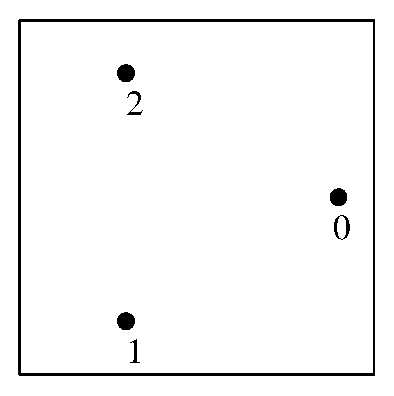
\includegraphics[width=2.5cm,angle=0]{getfemlist_intmethod_quad2.eps} & 
%   { \small
%     \begin{tabular}{m{3cm}m{3cm}}
%       $1/2+\sqrt{1/6}$ & $1/2$ \\ \\
%       $1/2-\sqrt{1/24}$ & $1/2\pm\sqrt{1/8}$ 
%     \end{tabular}
%     }
%   & 
%     \begin{tabular}{c}
%       1/3 \\ \\
%       1/3
%     \end{tabular}
%   & {\tt \small "IM\_QUAD(2)"} \hspace{11em} 3 points, order 2. \\ \hline
% \end{tabular}  
% \begin{tabular}{|m{2.5cm}|m{6cm}|m{1.2cm}|m{6.5cm}|}
%   \hline& & &\\ 
%   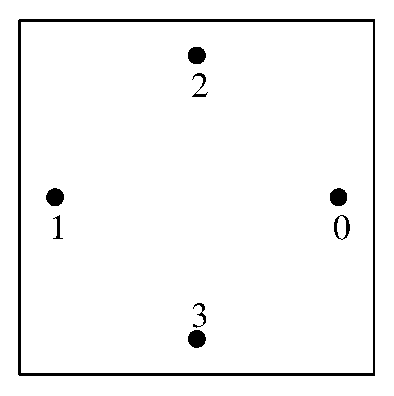
\includegraphics[width=2.5cm,angle=0]{getfemlist_intmethod_quad3.eps} & 
%   { \small
%     \begin{tabular}{m{3cm}m{3cm}}
%       $1/2\pm\sqrt{1/6}$ & $1/2$ \\ \\
%       $1/2$ & $1/2\pm\sqrt{1/6}$ 
%     \end{tabular}
%     }
%   & 
%     \begin{tabular}{c}
%       1/4 \\ \\
%       1/4
%     \end{tabular}
%   & {\tt \small "IM\_QUAD(3)"} \hspace{11em} 4 points, order 3. \\ \hline
% \end{tabular} 
% \begin{tabular}{|m{2.5cm}|m{6cm}|m{1.2cm}|m{6.5cm}|}
%   \hline& & &\\ 
%   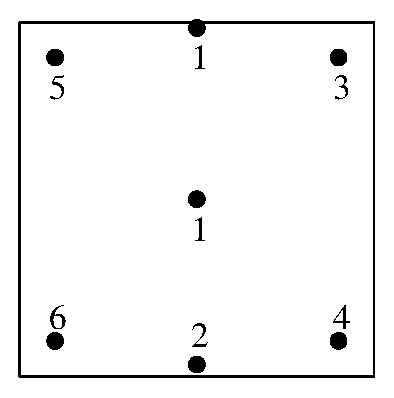
\includegraphics[width=2.5cm,angle=0]{getfemlist_intmethod_quad5.eps} & 
%   { \small
%     \begin{tabular}{m{3cm}m{3cm}}
%       1/2 & 1/2 \\ \\
%       $1/2 \pm \sqrt{7/30}$ & 1/2\\ \\
%       $1/2\pm\sqrt{1/12}$ & $1/2\pm\sqrt{3/20}$ 
%     \end{tabular}
%     }
%   & 
%     \begin{tabular}{c}
%       2/7 \\ \\
%       5/63 \\ \\
%       5/36
%     \end{tabular}
%   & {\tt \small "IM\_QUAD(5)"} \hspace{11em} 7 points, order 5. \\ \hline
% \end{tabular}  
% \begin{tabular}{|m{2.5cm}|m{6cm}|m{1.2cm}|m{6.5cm}|} \hline
% &&&{\tt \small "IM\_QUAD(7)"} \hspace{7em} \mbox{12 points, order 7}\hspace{7em} \\ \hline
% \end{tabular}
% \begin{tabular}{|m{2.5cm}|m{6cm}|m{1.2cm}|m{6.5cm}|} \hline
% &&&{\tt \small "IM\_QUAD(9)"} \hspace{7em} \mbox{20 points, order 9}\hspace{7em} \\ \hline
% \end{tabular}
% \begin{tabular}{|m{2.5cm}|m{6cm}|m{1.2cm}|m{6.5cm}|} \hline
% &&&{\tt \small "IM\_QUAD(17)"} \hspace{7em} \mbox{70 points, order 17}\hspace{7em} \\ \hline
% \end{tabular}
% ~\\[0.2cm]

% There is also the \cpp{IM\_GAUSS\_PARALLELEPIPED(n,k)} which is a direct product of 1D gauss integrations.\\

% \textbf{Important note:} do not forget that \cpp{IM\_QUAD(k)} is exact for polynomials up to degree $k$, and that a $Q_k$ polynomial has a degree of $2*k$. For example, \cpp{IM\_QUAD(7)} cannot integrate exactly the product of two $Q_{2}$ polynomials. On the other hand, \cpp{IM\_GAUSS\_PARALLELEPIPED(2,4)} can integrate exactly that product\ldots

% \subsection{Gauss Integration methods on dimension 3}

% \begin{tabular}{|m{2.5cm}|m{5.5cm}|m{1.2cm}|m{7.01cm}|} \hline 
% graphic & coordinates \hspace{5em} \begin{tabular}{m{1.7cm}m{1.7cm}m{1.7cm}} x & y & z \end{tabular} & weights & function to call / order \\ \hline
% \end{tabular}  
% \begin{tabular}{|m{2.5cm}|m{5.5cm}|m{1.2cm}|m{7.01cm}|}
%   \hline& & &\\ 
%   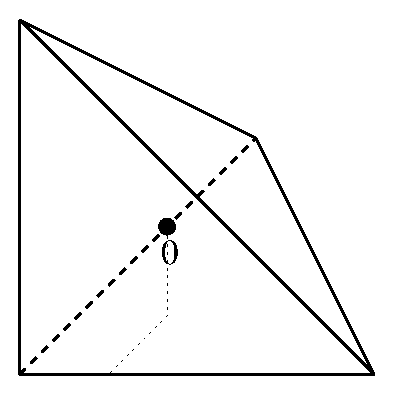
\includegraphics[width=2.5cm,angle=0]{getfemlist_intmethod_tetrahedron1.eps} & 
%   { \small
%     \begin{tabular}{m{1.7cm}m{1.7cm}m{1.7cm}}
%       $1/4$ & $1/4$ & $1/4$  
%     \end{tabular}
%     }
%   & 
%     { \small \begin{tabular}{c}
%       1/6
%     \end{tabular} }
%   & {\tt \small "IM\_TETRAHEDRON(1)"} \hspace{9em} 
%     1 point, order 1. \\ \hline
% \end{tabular}  
% \begin{tabular}{|m{2.5cm}|m{5.5cm}|m{1.2cm}|m{7.01cm}|}
%   \hline& & &\\ 
%   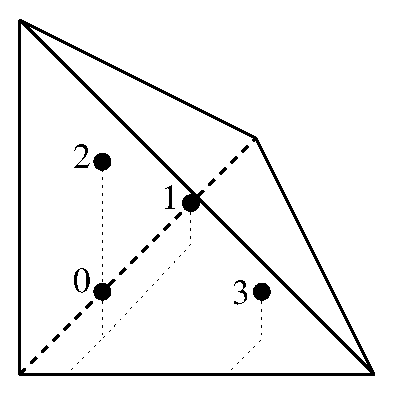
\includegraphics[width=2.5cm,angle=0]{getfemlist_intmethod_tetrahedron2.eps} & 
%   { \small
%     \begin{tabular}{m{1.7cm}m{1.7cm}m{1.7cm}}
%       $a$ & $a$ & $a$ \\
%       $a$ & $b$ & $a$ \\
%       $a$ & $a$ & $b$ \\
%       $b$ & $a$ & $a$ 
%     \end{tabular}
%     }
%   & 
%     { \small \begin{tabular}{c}
%       1/24 \\
%       1/24 \\
%       1/24 \\
%       1/24       
%     \end{tabular} }
%   & {\tt \small "IM\_TETRAHEDRON(2)"} \hspace{7em} 
%     \mbox{4 points, order 2} \hspace{7em}
%     \mbox{$a = \Frac{5 - \sqrt{5}}{20}$,}\hspace{5em}
%     \mbox{$b = \Frac{5 + 3\sqrt{5}}{20}$.}\hspace{5em} \hspace{5em} \hspace{5em}
%   \\ \hline
% \end{tabular}  
% \begin{tabular}{|m{2.5cm}|m{5.5cm}|m{1.2cm}|m{7.01cm}|}
%   \hline& & &\\ 
%   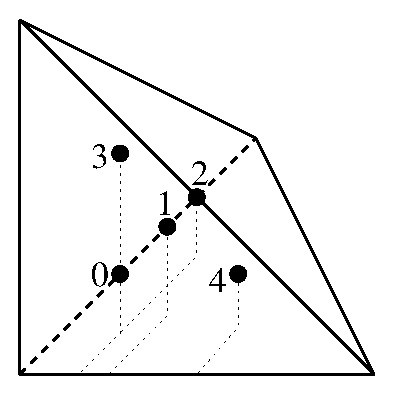
\includegraphics[width=2.5cm,angle=0]{getfemlist_intmethod_tetrahedron3.eps} & 
%   { \small
%     \begin{tabular}{m{1.7cm}m{1.7cm}m{1.7cm}}
%       $1/4$ & $1/4$ & $1/4$ \\
%       $1/6$ & $1/6$ & $1/6$ \\
%       $1/6$ & $1/2$ & $1/6$ \\
%       $1/6$ & $1/6$ & $1/2$ \\
%       $1/2$ & $1/6$ & $1/6$      
%     \end{tabular}
%     }
%   & 
%     { \small \begin{tabular}{c}
%       -2/15 \\
%       3/40 \\
%       3/40 \\
%       3/40       
%     \end{tabular} }
%   & {\tt \small "IM\_TETRAHEDRON(3)"} \hspace{7em} 
%     \mbox{5 points, order 3} \hspace{7em} \\ \hline
% \end{tabular}  
% \begin{tabular}{|m{2.5cm}|m{5.5cm}|m{1.2cm}|m{7.01cm}|}
%   \hline& & &\\ 
%   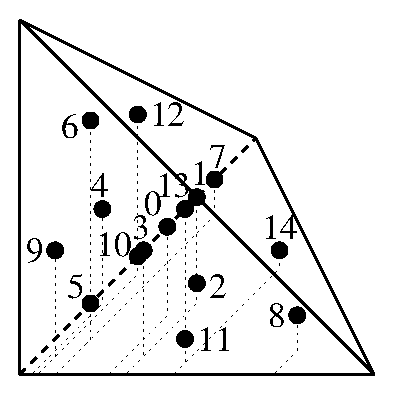
\includegraphics[width=2.5cm,angle=0]{getfemlist_intmethod_tetrahedron5.eps} & 
%   { \small
%     \begin{tabular}{m{1.7cm}m{1.7cm}m{1.7cm}}
%       $1/4$ & $1/4$ & $1/4$ \\
%       $a$ & $a$ & $a$ \\
%       $a$ & $a$ & $c$ \\
%       $a$ & $c$ & $a$ \\
%       $c$ & $a$ & $a$ \\ 
%       $b$ & $b$ & $b$ \\
%       $b$ & $b$ & $d$ \\
%       $b$ & $d$ & $b$ \\
%       $d$ & $b$ & $b$ \\
%       $e$ & $e$ & $f$ \\
%       $e$ & $f$ & $e$ \\
%       $f$ & $e$ & $e$ \\
%       $e$ & $f$ & $f$ \\
%       $f$ & $e$ & $f$ \\
%       $f$ & $f$ & $e$ 
%     \end{tabular}
%     }
%   & 
%     { \small \begin{tabular}{c}
%       8/405 \\
%       h \\
%       h \\
%       h \\
%       h \\      
%       i \\
%       i \\
%       i \\
%       i \\
%       5/567 \\
%       5/567 \\
%       5/567 \\
%       5/567 \\
%       5/567 \\
%       5/567
%     \end{tabular} }
%   & {\tt \small "IM\_TETRAHEDRON(5)"} \hspace{7em} 
%     \mbox{15 points, order 5} \hspace{7em}
%     \mbox{$a = \Frac{7 + \sqrt{15}}{34}$,}
%     \mbox{$b = \Frac{7 - \sqrt{15}}{34}$,}\hspace{5em}
%     \mbox{$c = \Frac{13 + 3\sqrt{15}}{34}$,}
%     \mbox{$d = \Frac{13 - 3\sqrt{15}}{34}$,}\hspace{5em}
%     \mbox{$e = \Frac{5 - \sqrt{15}}{20}$,}
%     \mbox{$f = \Frac{5 + \sqrt{15}}{20}$,}\hspace{5em}
%     \mbox{$h = \Frac{2665 - 14\sqrt{15}}{226800}$,}\hspace{5em} 
%     \mbox{$i = \Frac{2665 + 14\sqrt{15}}{226800}$,}\hspace{5em} 
%   \\ \hline
% \end{tabular}

% Others methods are:
% \begin{center}
%   \begin{tabular}{|lll|}
%     \hline name & convex type & nb of points\\
%     \hline \cpp{IM\_TETRAHEDRON(6)} & 3D simplex & 24\\
%     \cpp{IM\_TETRAHEDRON(8)} & 3D simplex & 43\\
%     \cpp{IM\_SIMPLEX4D(3)}   & 4D simplex & 6\\
%     \cpp{IM\_HEXAHEDRON(5)}  & 3D parallelepipeded & 14\\
%     \cpp{IM\_HEXAHEDRON(9)}  & 3D parallelepipeded & 58\\
%     \cpp{IM\_HEXAHEDRON(11)}  & 3D parallelepipeded & 90\\
%     \cpp{IM\_CUBE4D(5)}      & 4D parallelepipeded & 24\\
%     \cpp{IM\_CUBE4D(9)}      & 4D parallelepipeded & 145\\
%     \hline
%   \end{tabular}
% \end{center}
% \subsection{Direct product of integration methods}
% You can use {\tt "IM\_PRODUCT(IM1, IM2)"} to produce integration methods on quadrilateral or prisms. It gives the direct product of two integration mathods. For instance \cpp{IM\_GAUSS\_PARALLELEPIPED(2,k)} is an alias for \cpp{IM\_PRODUCT(IM\_GAUSS1D(2,k),IM\_GAUSS1D(2,k))} and ca be use instead of the \cpp{IM\_QUAD} integrations.

% \subsection{Composite integration methods}

% \begin{figure}[H]
%   \begin{center}
%     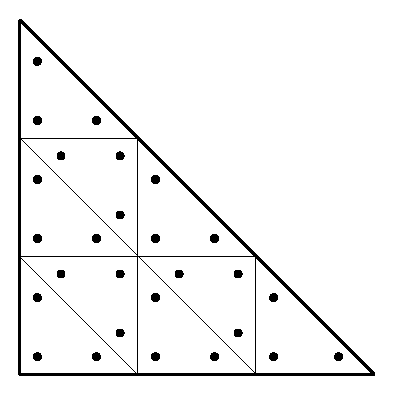
\includegraphics[width=5cm,angle=0]{getfemlist_intmethod_triangle2_comp.eps}
%   \end{center}
%   \caption{ \it composite method {\tt "IM\_STRUCTURED\_COMPOSITE(IM\_TRIANGLE(2), 3)"}} 
%   \label{fig:triangle_comp}
% \end{figure}


% use {\tt "IM\_STRUCTURED\_COMPOSITE(IM1, S)"} to copy {\tt IM1} on an element with {\tt S} subdivisions. The resulting integration method has the same order but with more points. This could be more stable to use composite method rather than to improve the order of the method. Those methods have to be used also with composite elements. Most of the time for composite element, it is preferable to choose the basic method {\tt IM1} with no points on the boundary (because the gradient coulb be not defined on the boundary of sub-elements). 


% For the HCT element, it is advised to use the \cpp{IM\_HCT\_COMPOSITE(im)} composite integration (which split the original triangle into 3 sub-triangles).







\section{Appendix C. Some basic computations between reference and real elements}
\subsection{Volume integral}
One has
\equat{\int_T f(x) dx = \int_{T'} f'(x') |\text{vol}\left(\Frac{\partial \tau(x')}{\partial x'_0} ;\Frac{\partial \tau(x')}{\partial x'_1}; ...; \Frac{\partial \tau(x')}{\partial x'_{P-1} }\right)| dx'.}
Denoting $J_{\tau}(x')$ the jacobian
\begin{center} \texonly{$ \fbox}{$\hspace{1em} J_{\tau}(x') := |\text{vol}\left(\Frac{\partial \tau(x')}{\partial x'_0} ;\Frac{\partial \tau(x')}{\partial x'_1}; ...; \Frac{\partial \tau(x')}{\partial x'_{P-1} }\right)| = (\mbox{det}(K(x')^T K(x')))^{1/2},\hspace{1em}$} \texonly{$}\end{center}
one finally has
\begin{center} \texonly{$ \fbox}{$\hspace{1em} \ds \int_T f(x) dx = \int_{T'} f'(x')  J_{\tau}(x')dx'.\hspace{1em}$} \texonly{$} \end{center}
When $P = N$, the expression of the jacobian reduces to $J_{\tau}(x') = |\mbox{det}(K(x'))|$.

\subsection{Surface integral}
With $\Gamma$ a part of the boundary of $T$ a real element and $\Gamma'$ the corresponding boundary on the reference element $T'$, one has
\begin{center} \texonly{$ \fbox}{$\hspace{1em} \ds \int_{\Gamma} f(x) d\sigma = \int_{\Gamma'} f'(x') \|B(x'){\mathbf n'}\| J_{\tau}(x') d\sigma',\hspace{1em}$} \texonly{$} \end{center}
where ${\mathbf n}'$ is the unit normal to $T'$ on $\Gamma'$. In a same way
\begin{center} \texonly{$ \fbox}{$\hspace{1em} \ds \int_{\Gamma} F(x).{\mathbf n} d\sigma = \int_{\Gamma'} F'(x').(B(x'){\mathbf n}') J_{\tau}(x') d\sigma'.\hspace{1em}$} \texonly{$} \end{center}

\subsection{Derivative computation}
One has
\equat{\nabla f(x) = B(x') \nabla'\,f'(x').}
\subsection{Second derivative computation}
Denoting 
\equat{\nabla^2 f = ({\Frac{\partial^2 f}{\partial x_i \partial x_j}})_{ij},}
the $N \times N$ matrix and
\equat{X'(x') = \sum_{k = 0}^{N-1} \nabla'^2 \tau_k(x') \Frac{\partial f}{\partial x_k}(x) = \sum_{k = 0}^{N-1} \sum_{i = 0}^{P-1} \nabla'^2 \tau_k(x') B_{ki} \Frac{\partial f'}{\partial x'_i}(x'),}
the $P \times P$ matrix, then
\equat{\nabla'^2 f'(x') = X'(x') + K(x')^T \nabla^2 f(x) K(x'),}
and thus
\equat{\nabla^2 f(x) = B(x') (\nabla'^2 f'(x') - X'(x')) B(x')^T.}

In order to have uniform methods for the computation of elementary matrices, the Hessian is computed as a column vector $H f$ whose components are $\Frac{\partial^2 f}{\partial x^2_0}, {\Frac{\partial^2 f}{\partial x_1 \partial x_0}}, ... {\Frac{\partial^2 f}{\partial x^2_{N-1}}}$.
Then, with $B_2$ the $P^2 \times P$ matrix defined as
\equat{(B_2(x'))_{ij} = \sum_{k = 0}^{N-1} \Frac{\partial^2 \tau_k(x')}{\partial x'_{i / P} \partial x'_{i \mbox{ mod } P} } B_{kj}(x'),}
and $B_3$ the $N^2 \times P^2$ matrix defined as
\equat{(B_3(x'))_{ij} = B_{i / N, j / P}(x') B_{i \mbox{ mod } N, j \mbox{ mod } P}(x'),}
one has
\begin{center} \texonly{$ \fbox}{ $H f(x) = B_3(x') \left(H'\,f'(x') - B_2(x')\nabla'\,f'(x')\right). $} \texonly{$} \end{center}

\subsection{Example of elementary matrix} \label{elmminst}

Assume one needs to compute the elementary ``matrix'':
\equat{t(i_0, i_1, ..., i_7) = \int_{T} \varphi_{i_1}^{i_0}\; \partial_{i_4} \varphi_{i_3}^{i_2}\; \partial^2_{i_7 / P, i_7 \mbox{ mod } P} \varphi_{i_6}^{i_5} dx,}
The computations to be made on the reference elements are
\equat{ t'_0(i_0, i_1, ..., i_7) = \int_{T'} \varphi'_{i_1}^{i_0}\; \partial_{i_4} \varphi'_{i_3}^{i_2}\; \partial^2_{i_7 / P, i_7 \mbox{ mod } P} \varphi'_{i_6}^{i_5}  J(x') dx',}
and
\equat{t'_1(i_0, i_1, ..., i_7) = \int_{T'} \varphi'_{i_1}^{i_0}\; \partial_{i_4} \varphi'_{i_3}^{i_2}\; \partial_{i_7} \varphi'_{i_6}^{i_5}  J(x') dx',}
Those two tensor can be computed once on the whole reference element if the geometric transformation is linear (because $J(x')$ is constant). If the geometric transformation is non-linear, what has to be stored is the value on each integration point. To compute the integral on the real element a certain number of reductions have to be made:
\begin{itemize}
    \item Concerning the first term ($\varphi_{i_1}^{i_0}$) nothing.
    \item Concerning the second term ($\partial_{i_4} \varphi_{i_3}^{i_2}$) a reduction with respect to $i_4$ with the matrix $B$.
    \item Concerning the third term ($\partial^2_{i_7 / P, i_7 \mbox{ mod } P} \varphi_{i_6}^{i_5}$) a reduction of $t'_0$ with respect to $i_7$ with the matrix $B_3$ and a reduction of $t'_1$ with respect also to $i_7$ with the matrix $B_3B_2$
 \end{itemize}
 The reductions are to be made on each integration point if the geometric transformation is non-linear. Once those reductions are done, an addition of all the tensor resulting of those reductions is made (with a factor equal to the load of each integration point if the geometric transformation is non-linear).

 If the finite element is non-$\tau$-equivalent, a supplementary reduction of the resulting tensor with the matrix $M$ has to be made.



\begin{thebibliography}{99}
% \bibliographystyle{apalike}
% \bibliographystyle{plain}
% \bibliography{all}

\bibitem{bank1983}
  R.E. {\texonly{\sc} Bank, A.H. Sherman, A. Weiser}
  {\it Refinement algorithms and data structures for regular local mesh refinement},
  in Scientific Computing IMACS, Amsterdam, North-Holland, pp 3-17, 1983

\bibitem{ciarlet1978}
  P.G.. {\texonly{\sc} Ciarlet},
  {\it The finite element method for elliptic problems}, Studies in Mathematics and its Applications vol. 4, North-Holland, 1978.

\bibitem{dh-to1984} 
  {\texonly{\sc} G. Dhatt, and  G. Touzot}
  {\it The Finite Element Method Displayed}, 
  J. Wiley \& Sons,  New York, 1984.

\bibitem{EncyclopCubature}
  R. {\texonly{\sc} Cools}
  {\it An Encyclopaedia of Cubature Formulas}, J. Complexity, \cpp{http://www.cs.kuleuven.ac.be/\tilda ines/research/ecf/ecf.html}
  
\bibitem{Xfem}
  N. {\texonly{\sc} Mo�s, J. Dolbow and T. Belytschko}
  {\it A finite element method for crack growth without remeshing },
  Int. J. Num. Meth. Engng. 46, 131-150 (1999).  

\bibitem{nedelec1991}
  J.-C. {\texonly{\sc} Nedelec},
  {\it Notions sur les techniques d'{\'e}l{\'e}ments finis}, Ellipses, SMAI, Math{\'e}matiques \& Applications n$^o7$, 1991.

\bibitem{so-se-do2004}
  P. {\texonly{\sc} Solin, K. Segeth, I. Dolezel},
  {\it Higher-Order Finite Element Methods}, Chapman and Hall/CRC, Studies in advanced mathematics, 2004.

\end{thebibliography}

% \W \section*{Index}
% \texorhtml{\printindex}{\label{gfmindex}\htmlprintindex}

\end{document}
